\documentclass[conference]{IEEEtran}
\usepackage{threeparttable}
% === Packages ===
\usepackage{pgfplots}
\usepackage{tikz}
\usepackage{etex}
\usepackage{graphicx}
%\usepackage{algorithm}
\usepackage[linesnumbered,ruled,vlined]{algorithm2e}
\usepackage{booktabs}
\usepackage{algpseudocode}
\usepackage{smartdiagram}
\algrenewcommand\Call[2]{\textsc{#1}(#2)}   
\usepackage{amsmath}
\usepackage{amsthm}
\usepackage{tikzpagenodes}
\usepackage{tabularx}
\usepackage{xcolor}
\usepackage{amssymb}
\usepackage{pifont}
\usepackage{xspace}
\usepackage[normalem]{ulem}
\usepackage{subfigure}
\usepackage{cite}
\usepackage{url}
\usepackage[dvipsnames]{xcolor}
\usepackage[hidelinks]{hyperref}   
\usepackage{tcolorbox}
\usepackage{comment}
\tcbuselibrary{breakable}
% === TikZ Libraries ===
\usetikzlibrary{shapes,patterns,calc,arrows,arrows.meta,positioning,fit,backgrounds,shadows.blur,decorations}

% === Theorems ===
\newtheorem{theorem}{Theorem}
\newtheorem{lemma}{Lemma}

% === Custom Commands ===
\newcommand{\cmark}{\ding{51}}
\newcommand{\xmark}{\ding{55}}
\newcommand{\BfPara}[1]{\vspace{1mm}{\noindent\textbf{#1.}}\xspace}

\newcommand*\circled[1]{\tikz[baseline=(char.base)]{
            \node[shape=circle, fill=black,text=white, draw,inner sep=0.25pt] (char) {\bfseries #1};}}

\newcommand{\textbox}[2][]{%
  \begin{tcolorbox}[colback=white, colframe=black,
                    boxrule=0.5pt, arc=1mm, breakable, boxsep=2pt, left=1pt, right=1pt, top=1pt, bottom=1pt,  before skip=4pt, after skip=4pt, width=\linewidth, #1]
    #2
  \end{tcolorbox}%
}

\newcommand{\rj}[1]{{\color{blue}#1}}
\newcommand{\yiwen}[1]{{\color{ForestGreen}#1}}
\newcommand{\os}[1]{{\color{teal}#1}}
\newcommand{\anik}[1]{{\color{violet}#1}}
\newcommand{\md}[1]{{\color{purple}#1}}

\bibliographystyle{IEEEtran}

% =============================================================================
\begin{document}
% =============================================================================

\title{BGP-Sentry: Extending the RPKI Root of Trust to Non-Participating Networks}
\author{Anonymous authors}

% --- Draft navigation aids (remove before submission) ---
%\tableofcontents
%\listoffigures
%\listoftables
%\newpage
% --- End draft aids ---

\maketitle

% === Abstract ===
\begin{abstract}
The current landscape of secure BGP is characterized by a fundamental trust asymmetry. RPKI provides a beacon of trust for its members; however, the majority of the Internet remains a dark, unverifiable periphery. While universal adoption remains practically unfeasible, the resulting lack of cryptographic visibility into these regions creates an unaddressed systemic risk.

BGP-Sentry resolves this stalemate by transforming RPKI-enabled networks into authoritative observers. The core insight is transitive: while we cannot verify the claims of a network without an RPKI identity, we can cryptographically verify the observations of their behavior made by those who have one. By anchoring these attestations to the RPKI root, BGP-Sentry creates a longitudinal Behavioral Attestation Index (BAI). This framework evolves the Internet from simple identity validation toward collective accountability, allowing the trust of the RPKI core to illuminate the entire routing landscape. BGP-Sentry enables active, risk-aware filtering, securing the global Internet using the trust we already have.
\end{abstract}

\begin{IEEEkeywords}
Border Gateway Protocol, Resource Public Key Infrastructure, Route Origin Authorization, Blockchain.
\end{IEEEkeywords}

\IEEEpeerreviewmaketitle

% === Main Body ===
% §1 Introduction          - Problem, contributions, paper outline
% §2 Background/Motivation - Challenges, why existing solutions fail
% §3 Proposed Architecture - System design, consensus, algorithms
% §4 Security Enforcement  - Attack detection pipeline, penalties
% §5 System Evaluation     - Dataset, results (correctness, scalability, security utility)
% §6 Discussion            - Interpretation, limitations, future work
% §7 Related Work          - Comparison with prior approaches
% §8 Conclusion








\section{Introduction}
\label{sec:introduction}

The Border Gateway Protocol (BGP) is the foundational protocol that enables inter‐domain routing across tens of thousands of Autonomous Systems (ASes)~\cite{rfc4271}. The inter‐domain BGP validation and filtering, introduced in 1995, have relied on the Internet Routing Registry (IRR)~\cite{DuIRATSc23}, a public database that allows operators to publish IP‐prefix/ASN pairs, with each prefix authorized to originate from a given ASN. Nevertheless, IRRs provide neither strong publisher authentication nor cryptographic guarantees of prefix ownership, leading to persistent risks of misinformation or misconfiguration~\cite{MahajanWA02,KangLRKC24IRRedicator,DuIRATSc23}. Moreover, conflicting data across multiple IRRs creates loopholes that adversaries can exploit to bypass route‐monitoring filters~\cite{BirgeLeeAR25}.
The absence of a native authentication mechanism exposes BGP to a wide range of attacks, including hijacking~\cite {prefixHijacking} and leakage~\cite {McDanielSS21BGPLeak}, resulting in severe disruptions, such as traffic blackholing, interception, or global outages~\cite{butler2009survey}. \rj{To provide stronger security, BGPsec~\cite{rfc8205BGPSec} introduces a cryptographic trust model for path validation, but its adoption remains very low, near zero~\cite{}, due to the complex computing required on the resource-constrained data plane and the requirement for simultaneous adoption across the routing path. }



%Recent work demonstrates that even RPKI-protected networks remain vulnerable to update-message flooding attacks that induce route oscillations that can destabilize large portions of the Internet~\cite{stoger2025vortex}.

\rj{As a more practical and widely adopted alternative, Resource Public Key Infrastructure (RPKI) \cite{RPKI} provides a foundation for Route Origin Authorization (ROA). However, even RPKI’s effectiveness is limited by its binary nature (\texttt{VALID} and \texttt{INVALID}) and incomplete global adoption, with only 38.7\%~\cite{qin2024understanding} of ASes currently enforcing validation. This leaves the Internet as a fragmented landscape where trust is frequently broken at the boundary between protected and unprotected networks.}




\begin{figure}[t]
    \centering 
    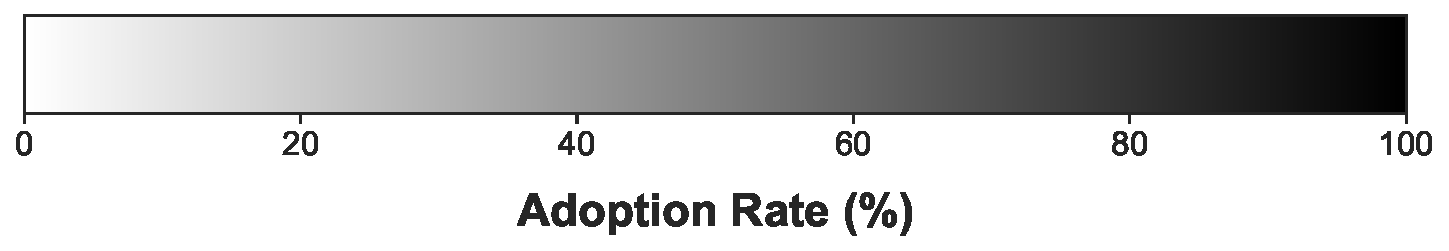
\includegraphics[width=0.3\textwidth]{figures/ROV_legend.pdf}\vspace{-1mm}
  \subfigure[IPv4]{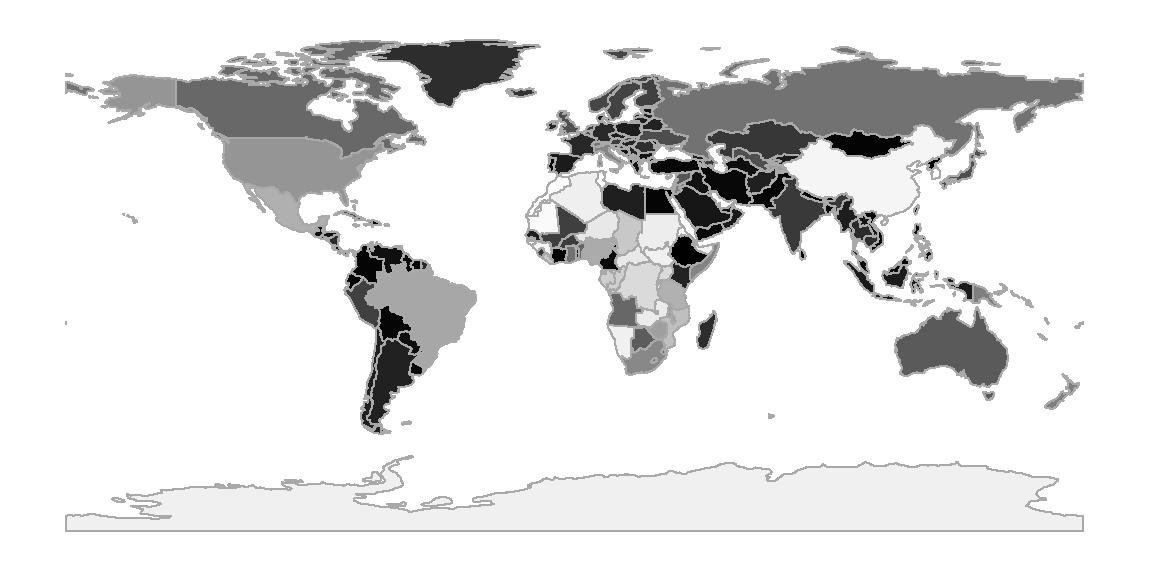
\includegraphics[width=0.23\textwidth, height=2.5cm]{figures/ROV_IPv4.pdf}}\hspace{1mm}
    \subfigure[IPv6]{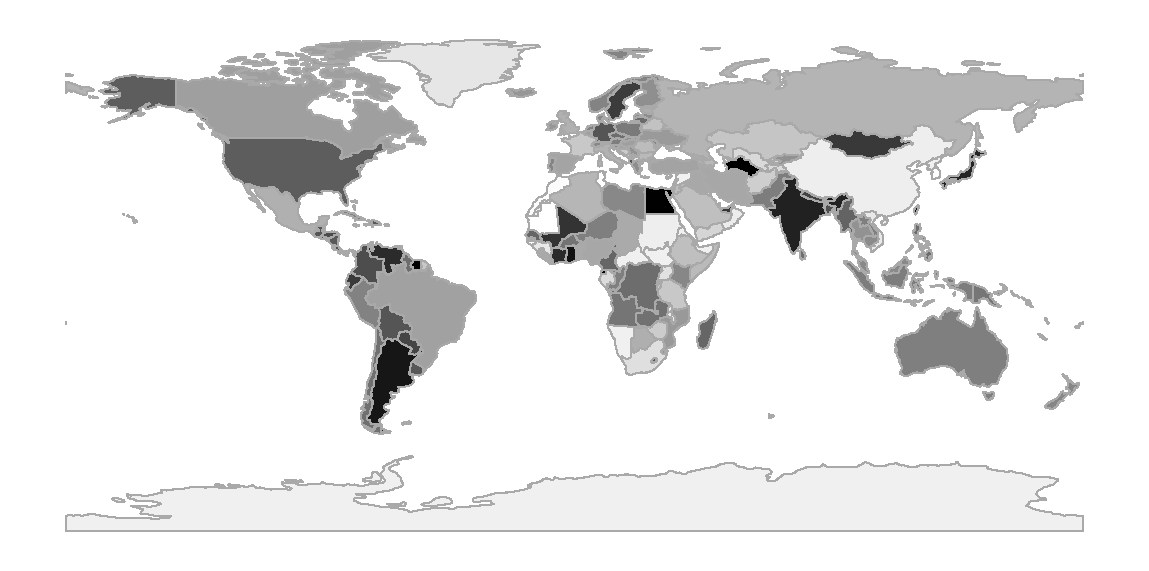
\includegraphics[width=0.23\textwidth, height=2.5cm]{figures/ROV_IPv6.pdf}}%\vspace{-3mm}
    \caption{\rj{Distribution of RPKI adoption across IPv4 and IPv6 prefixes. The data highlights the fragmented nature of current BGP security, where the majority of the Internet lacks native cryptographic protection.}}
    \label{fig:IP_rov}
\end{figure}



Although existing research has criticized RPKI's centralized trust model and its complex fetching and caching mechanisms~\cite{HlavacekSVW23BGPAdopt}, and recent systematization reveals that 56\% of RPKI validators contain implementation vulnerabilities exploitable for Denial of Service (DoS) threats~\cite{stoger2025vortex, mirdita2025sok}, \rj{raising \textbf{single-point failure} concerns. 
To address the issue, recent efforts have turned to blockchain-based architectures~\cite{saad2022routechain, chen2020isrchain}, attempting to decentralize trust for resiliency. Nevertheless, there still three core questions remain unanswered for practical and wide deployment of  RPKI in practice:}

\textbox{\textbf{RQ1) Bridging the Trust and Deployment Gap.} How can the cryptographic root of trust from the RPKI ecosystem be transitively extended to provide verifiable security for the 41.4\% of the Internet that remains outside the RPKI periphery?}
%\textbf{(RQ1) Bridging the Deployment Gap.} \rj{How can the cryptographic root of trust from the RPKI ecosystem be transitively extended to provide verifiable security for the 63\% of the Internet that remains outside the RPKI periphery?}

Despite significant progress in prefix signing, where 49.8\% of IPv4 and 48.13\% of IPv6 prefixes are now covered by valid ROAs \cite{nro2026rpki}, a critical enforcement gap remains. \yiwen{The majority of the Internet still operates without active RPKI-based validation on BGP sessions, meaning that even when cryptographic records exist, they are frequently ignored during route selection}~\cite{qin2024understanding}. 
Consequently, large portions of the Internet remain unable to programmatically validate incoming announcements, effectively preventing the RPKI trust anchor from influencing routing decisions at the network edge.
% This leaves the remainder of the ecosystem unable to programmatically verify incoming announcements, rendering the existing cryptographic root ineffective at the network edge. 
Furthermore, existing hybrid approaches that bridge this gap by combining \textit{RPKI} with legacy \textit{IRR} filtering \cite{KangLRKC24IRRedicator} continue to suffer from the weak authentication inherent in IRR databases, thereby introducing additional attack vectors rather than resolving the underlying trust deficit.

\textbox{\textbf{RQ2) Establishing a Trustworthy Audit Trail.} How can a decentralized and immutable ledger be designed to transform transient BGP routing observations into a practical and reliable audit trail of AS behavior?}


Existing blockchain-based BGP security solutions, such as RouteChain~\cite{saad2022routechain} and ISRchain~\cite{chen2020isrchain}, fail to provide a reliable audit trail due to two structural deficiencies. \rj{First, they \textit{lack topological alignment}.} 
\os{RouteChain, for example, groups ASes based on geographical proximity rather than actual peering and transit relationships, leading to audit records that distort the true path of trust propagation.}
% RouteChain groups ASes by geographical proximity rather than functional peering relationships, resulting in an audit record that misinterprets the path of trust.
\rj{Second, they suffer from a \textit{data integrity gap}.} By relying on passive logging without cryptographically anchoring observers to the RPKI root, these systems cannot verify the authority of the entity reporting a routing event. Consequently, their ledgers remain collections of unverified, fragmented snapshots rather than a continuous, authoritative history capable of supporting longitudinal behavioral analysis.

\textbox{\textbf{RQ3) Enabling Closed-loop Security Enforcement.} What is the missing link that can effectively translate decentralized behavioral audits into active and secure routing enforcement?}


% The RPKI framework (RFC 6480~\cite{RPKI}) provides transient origin validation but lacks a standardized mechanism for longitudinal state retention.
The RPKI framework (RFC~6480~\cite{RPKI}) enables cryptographic route origin validation but is inherently \textit{stateless}, providing only transient assessments of individual announcements without retaining longitudinal context. 
This creates an \rj{\textit{enforcement blind spot}} without a verifiable record of past behavior; thereby, operators cannot differentiate between isolated misconfigurations and persistent malicious hijacking. Consequently, there is a critical need for an RPKI-based architecture that: 1) transforms transient observations into a persistent, verifiable audit trail, and 2) translates this behavioral history into \rj{automated and trust-based enforcement policies} that extend security guarantees even to non-RPKI networks.




\rj{Our answer to the above-mentioned research questions and challenges is BGP-Sentry, a blockchain-based trust-expansion framework that transforms RPKI-enabled ASes into distributed observers of their neighbors. By recording observed BGP behaviors on a shared ledger rooted in the foundational trust of the central RPKI, these events are used to compute a longitudinal Behavioral Attestation Index (BAI) for each AS (both RPKI-enabled and non-RPKI) through protocol-embedded algorithms executed during blockchain consensus.}

\noindent \textbf{(i) Resolving Isolation via Hierarchical Chain of Trust.} 
\rj{We resolve the cryptographic opacity and ``isolated world'' problem of non-RPKI networks by designing a multi-layered chain of trust that extends the cryptographic authority of the Central RPKI to the previously opaque non-RPKI regions. By anchoring blockchain identities to RPKI certificates, the framework establishes a verifiable provenance for all routing attestations, allowing RPKI-enabled ASes to act as ``trust proxies'' and enabling authoritative attribution and forensic accountability for 41\% of the Internet currently lacking native cryptographic protection.}

\noindent \textbf{(ii) Scaling Up Identity-based Blockchain Consensus.} 
\rj{We resolve the scalability bottlenecks of identity-based blockchains, specifically $O(n^2)$ communication complexity and recursive validation overhead, by introducing a \textit{Data Plane-aware Proof of Population} (DP-PoP) consensus anchored to the RPKI hierarchy. By restricting the validator set to verified and neighbour ASes within a few hops, BGP-Sentry achieves sub-linear overhead growth and negligible consensus latencies. This foundation supports a collaborative behavioral monitoring ecosystem, effectively extending the RPKI root of trust to 41\% of non-RPKI networks to create a proactive, self-defending routing infrastructure.}

\noindent \textbf{(iii) Blockchain Attestation to Active Routing Enforcement.} 
\rj{We propose a robust framework for inter-domain accountability by synthesizing diverse BGP signals, including announcement consistency, reverse-path verification, and registry cross-checking, into a longitudinal \textit{Behavioral Attestation Index (BAI)}. Unlike transient reputation scores, the BAI captures long-term protocol integrity through protocol-embedded algorithms executed during blockchain consensus. We demonstrate the utility of this framework through a qualitative five-tier trust classification (from \texttt{Highly Trusted} to \texttt{Malicious}), providing RPKI-compliant operators with an immutable audit trail and a deterministic basis for risk-aware routing decisions when interfacing with the 41\% of non-RPKI domains.}

\rj{The design goal of BGP-Sentry is to \textit{illuminate the global AS topology} by extending the reach of cryptographic trust to the previously opaque regions of the Internet. Currently, the inter-domain landscape is a fragmented ``isolated world,'' split between the RPKI-protected core and a vast unverifiable periphery. Technically, we bridge this paradox, expanding the ``trust'' of the Central RPKI to unify these disconnected domains into a single, accountable routing ecosystem.}

% \noindent \textbf{(iv) Incentive-Compatible Monitoring via BGP Coins.} 
% \rj{We ensure the long-term viability of the decentralized framework by introducing \textit{BGP Coins}, a participation incentive that replaces operator altruism with tangible rewards for active observation. By aligning the economic interests of RPKI-enabled ASes with global security goals, this mechanism fosters the collective monitoring power necessary to bridge isolated routing domains into a unified, accountable, and self-defending ecosystem.}



\section{Preliminary}
\subsection{BGP Vulnerabilities and RPKI Architecture}
\yiwen{The Border Gateway Protocol (BGP) exchanges routing information via UPDATE messages containing Network Layer Reachability Information (NLRI) and path attributes like AS\_PATH~\cite{lougheed1990rfc1163}. Lacking native cryptographic origin authentication, BGP is fundamentally vulnerable to forged NLRIs. In a prefix hijacking attack~\cite{prefixHijacking}, a malicious Autonomous System (AS) exploits the BGP decision process by announcing a more specific prefix (leveraging the Longest Prefix Match rule) or synthesizing an artificially short AS\_PATH to intercept traffic.}

\yiwen{Early mitigation efforts like BGPsec~\cite{rfc8205BGPSec} proposed an inline security extension. BGPsec requires each transit AS to cryptographically sign the routing update using an ECDSA signature covering the NLRI, the AS\_PATH, and the target AS. However, BGPsec failed to gain traction due to prohibitive technical barriers: wire-speed validation of nested ECDSA signatures strains routing hardware, and its strict sequential validation requirement renders partial deployment ineffective.}

\yiwen{To bypass these constraints, the networking community adopted the Resource Public Key Infrastructure (RPKI)~\cite{RPKI}. RPKI operates entirely out-of-band, separating the cryptographic security layer from the routers making packet-forwarding decisions. Its architecture follows a distinct workflow:}

\yiwen{\begin{enumerate}
    \item \textbf{Trust Anchors and Certificates:} The global IP address space is managed by five Regional Internet Registries (RIRs). Acting as Trust Anchors, RIRs issue X.509 certificates (with RFC 3779 extensions) that cryptographically bind allocated IP blocks and ASNs to an organization's public key.
    
    \item \textbf{Route Origin Authorization (ROA):} Using this certificate, the resource holder generates a ROA~\cite{rfc6482}. A ROA is a signed object that authorizes a specific ASN to originate a designated IP prefix. It includes a \textit{maxLength} attribute specifying the most specific permitted subnet, mitigating attacks that exploit Longest Prefix Match routing.
    
    \item \textbf{Validation and Enforcement:} Network operators deploy standalone software known as Relying Parties (RPs) within their local infrastructure. These RP caches perform the computationally heavy tasks: fetching, cryptographically validating, and caching ROAs from global repositories. Local edge routers then utilize the RPKI-to-Router (RTR) protocol~\cite{rfc6810} to download a streamlined list of Validated ROA Payloads (VRPs) and perform Route Origin Validation (ROV), dropping invalid BGP announcements.
\end{enumerate}}

\subsection{Blockchain-based RPKI and Proof-of-Population}
\begin{comment}
\yiwen{While RPKI resolves router computational overhead, its strict top-down hierarchy introduces structural vulnerabilities. The reliance on centralized RIRs creates Single Points of Failure (SPOFs); misconfigurations, compromised Trust Anchors, or unilateral certificate revocations can instantly invalidate legitimate routing states globally~\cite{nro2026rpki}.}

\yiwen{To mitigate these centralized risks, recent literature advocates for a decentralized Public Key Infrastructure (dPKI) utilizing blockchain. By mapping IP prefix allocation and AS identity to on-chain smart contracts, routing states transform into an immutable ledger governed by distributed consensus, removing the reliance on centralized dictates.}

\yiwen{Securing this permissionless ledger requires robust, Sybil-resistant consensus algorithms. Traditional Proof-of-Work (PoW) introduces unacceptable latency and energy overhead for dynamic routing updates. Instead, Proof-of-Population (PoP) provides a structurally aligned alternative. PoP binds on-chain voting power directly to cryptographically verified, unique entities rather than hash rates. This enforces a strict ``one-entity, one-vote'' governance model, neutralizing Sybil attacks where an adversary synthesizes fake identities to hijack consensus. While systems like RouteChain~\cite{saad2022routechain} and ISRchain~\cite{chen2020isrchain} utilize distributed ledgers to anchor routing updates, resolving on-chain state bloat and cross-chain interoperability remains an ongoing challenge.}
\end{comment}
% From Nyang to Anik and Yiwen: I have further developed the draft by incorporating the part Yiwen wrote, including the commented-out section. If you think any part should be revised, or if the text is too long and needs to be condensed, please feel free to adjust it as you want.
While RPKI resolves router computational overhead by moving expensive cryptographic validation out of the forwarding path, its strict top-down hierarchy introduces structural vulnerabilities. The reliance on centralized RIRs creates Single Points of Failure (SPOFs); misconfigurations, compromised Trust Anchors, or unilateral certificate revocations can instantly invalidate legitimate routing states globally~\cite{nro2026rpki}. To mitigate these centralized risks, recent literature advocates for a decentralized Public Key Infrastructure (dPKI) utilizing blockchain. By mapping IP prefix allocation and AS identity to on-chain smart contracts, routing states transform into an immutable ledger governed by distributed consensus, reducing reliance on centralized dictates. However, for such a ledger to be practical in the inter-domain routing environment, the consensus mechanism must not only provide integrity, but also align with the identity and observability properties of BGP.

A useful foundation for such a design is Proof-of-Population (PoP), originally introduced in Gruut as a low-cost, signature-based alternative to Proof-of-Work (PoW)~\cite{nyang2018gruut}. In PoP, consensus is achieved not through hashpower competition, but through the accumulation of endorsements from identified participants. A block becomes valid when an eligible producer gathers a predefined number of signatures, and in the presence of contention, the preferred chain is the one supported by the larger accumulated population. By binding voting power to verifiable entities rather than computational resources, PoP realizes a practical ``one-entity, one-vote'' model, reduces consensus cost, makes double voting attributable, and makes secret fork construction substantially harder because conflicting histories require visible collaboration from other signers~\cite{nyang2018gruut}.

Securing a permissionless routing ledger requires a consensus mechanism that is not only Sybil-resistant, but also compatible with the operational characteristics of inter-domain routing. Traditional Proof-of-Work (PoW) introduces unacceptable latency and energy overhead for dynamic BGP updates, making it ill-suited to this setting. Although prior systems such as RouteChain~\cite{saad2022routechain} and ISRchain~\cite{chen2020isrchain} employ distributed ledgers to anchor routing information, important challenges remain, including on-chain state bloat, interoperability, and, most importantly, the lack of a routing-aware consensus model. In this respect, PoP offers a more structurally aligned alternative. By binding on-chain voting power to cryptographically verified, unique entities rather than hash rates, PoP enforces a practical one-entity-one-vote model and naturally resists Sybil attacks. Its signature-based, low-cost consensus mechanism is therefore well matched to a routing environment in which authenticated entities collaboratively validate observed events rather than compete through computational expenditure~\cite{nyang2018gruut}.

% Building on this intuition, TrustChain adapts PoP to the BGP setting rather than using it unchanged. First, identity is grounded not in general real-world identification, but in \emph{RPKI-verified AS identity} established during onboarding, so that a participant enters the consensus set only after proving control over its certificate chain and ROA-related cryptographic material. Second, the consensus object is not a financial transaction block, but a \emph{BGP observation} generated by an RPKI-enabled observer. Third, because BGP exhibits \emph{asymmetric visibility}, where routing updates are observable only to topologically relevant neighbors and path-adjacent participants, validator selection must also follow routing visibility rather than global randomization. Accordingly, TrustChain employs a \emph{Data Plane-aware Proof-of-Population (DP-PoP)} model, in which observers seek endorsements only from RPKI-enabled peers with meaningful vantage points over the event, and record the observation once it accumulates the quorum threshold $\tau$. As a result, TrustChain preserves the main advantage of PoP, identity-bound, population-backed, low-cost signature consensus, while avoiding blind voting and reducing unnecessary communication overhead. The blockchain, therefore, functions not only as a decentralized registry, but also as a \emph{behavioral attestation layer} that transforms transient routing observations into persistent, verifiable, and consensus-backed evidence, enabling longitudinal trust scoring and active security enforcement against both RPKI-participating and non-participating networks.


\iffalse
\subsection{The Road to RPKI: Securing the BGP Ecosystem}
\md{The Border Gateway Protocol (BGP) has served as the basis for the Internet's routing for decades~\cite{lougheed1990rfc1163}, designed primarily for global reachability via flexible, policy-driven path selection. However, BGP’s initial design prioritized scalability and autonomy over security, assuming an implicit trust model in which route announcements are accepted without verification. This architectural gap has led to serious vulnerabilities, such as prefix hijacking~\cite{prefixHijacking} and route leaks~\cite{McDanielSS21BGPLeak}, where malicious or misconfigured ASes redirect traffic by claiming unauthorized ownership of IP resources.}

\md{Early efforts to secure BGP, such as BGPsec~\cite{rfc8205BGPSec}, aimed to provide full-path validation but failed to gain traction due to high computational overhead, significant hardware requirements, and the ``all-or-nothing'' nature of its deployment. Consequently, the networking community shifted its focus toward the Resource Public Key Infrastructure (RPKI)~\cite{RPKI}. Similar to the Web PKI used for SSL/TLS, RPKI provides a cryptographically verifiable hierarchy that roots Internet resources (IP addresses and ASNs) in a chain of trust managed by the five Regional Internet Registries (RIRs).}

\md{Under this framework, network resource owners register their prefixes by creating RPKI objects, most notably the Route Origin Authorization (ROA). An ROA is a digitally signed record that explicitly maps a specific IP prefix to its authorized origin AS for prefix announcement. Since its standardization in 2012, RPKI has become the primary mechanism for Route Origin Validation (ROV). However, as the global routing landscape evolves, the transition to RPKI becomes difficult~\cite{KangLRKC24IRRedicator, testart2020filter, nro2026rpki}. Therefore, recent research focuses on improving RPKI adoption by reducing deployment overhead~\cite{chung2019rpki, ni2025address}, mitigating operational risks~\cite{li2025improv, chen2025right}, and extending security beyond simple origin validation~\cite{hoger2025xbgpsec, rfc9234}.}


\subsection{Decentralized Trust: Blockchain Model}
\md{Blockchain is a distributed ledger technology (DLT) that maintains a shared and unchangeable record of events across a peer-to-peer network. At its core, it provides immutability, transparency, and decentralized consensus, enabling a tamper-evident, publicly auditable system without reliance on a central authority. To function without a central authority, the network follows a consensus mechanism, which defines a set of rules that ensure that all participants agree on the state of the ledger. Common types include Proof-of-Work (PoW), which relies on computational power, and Proof-of-Population (PoP), which enforces a ``one-entity, one-vote'' model through a strict identity verification process to prevent any single participant from unfairly influencing the ledger.}

\md{The decentralized and auditable properties of blockchain have motivated its use as a security layer for the Internet's routing infrastructure, BGP. Since BGP is inherently a decentralized ``network of networks'', a shared ledger naturally reflects the Internet's topology. Recent studies, including RouteChain~\cite{saad2022routechain} and ISRchain~\cite{chen2020isrchain}, demonstrate how blockchain can track routing updates and maintain a verifiable temporal history of prefix ownership. However, while these works demonstrate the potential for decentralized trust, they face significant structural and operational limitations.}
\fi



\section{Motivating BGP-Sentry}\label{sec:motivation}

Securing trust in the BGP protocol presents multifaceted challenges that existing solutions do not address. Although RPKI has been proposed as a potential solution, it alone is not sufficient to achieve robust BGP security. We identify three critical challenges that explain why current approaches, including RPKI and blockchain-based solutions, leave BGP vulnerable. These limitations motivate our work to design BGP-Sentry, a blockchain-based trust-expansion framework.


\begin{figure}
    \centering
    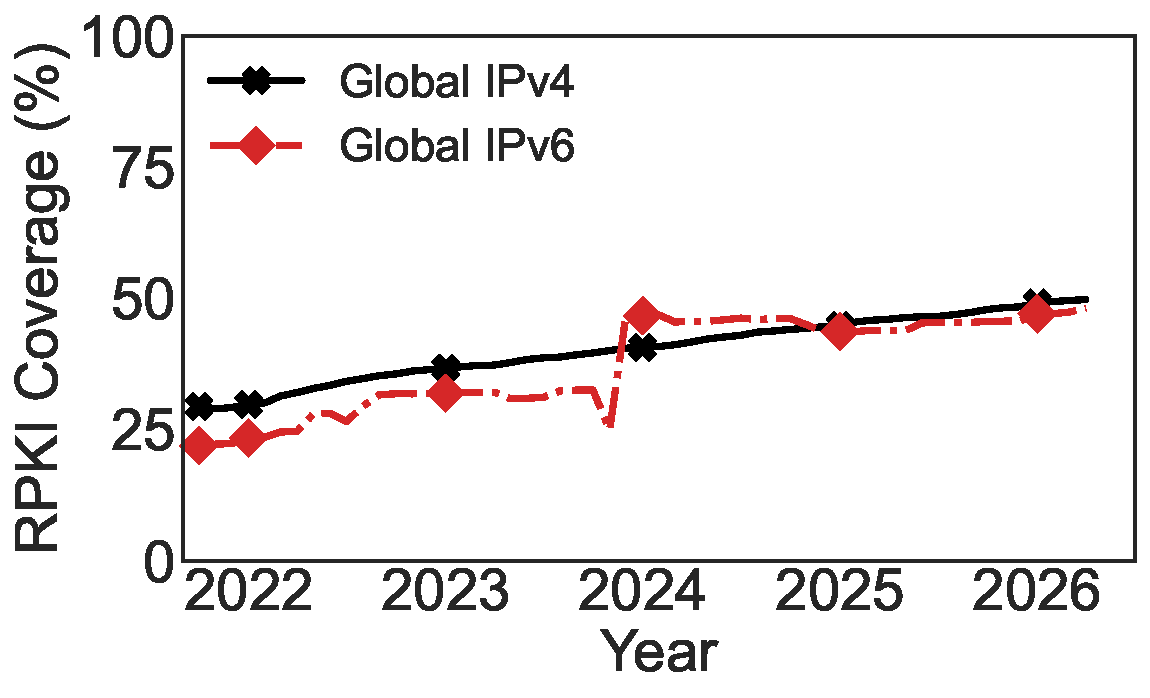
\includegraphics[width=0.35\textwidth]{figures/Global_RPKI.pdf}
    \caption{Global RPKI adoption trends: growth of ROA-protected address space in IPv4 and IPv6 over the last 5 years.}
    \label{fig:RPKI_cov}
\end{figure}

\subsection{Analysis of Universal RPKI Deployment} 

\md{With over 79,000 Autonomous Systems (ASes) on the Internet, only 58.6\%~\cite{caida-dataset} have adopted RPKI. Figure~\ref{fig:RPKI_cov} shows the slow RPKI coverage trend for both IPv4 and allocated IPv6 space (excluding reserved IP addresses) over the last five years, based on monthly snapshots from the NRO (Number Resource Organization)~\cite{nro2026rpki}, which tracks the global progress of ROA-protected resources. As shown, despite RPKI adoption by more than half of ASes, they collectively protect only 49.8\% of the total IPv4 space and 48.1\% of IPv6 as of April 1st, 2026.  Additionally, a recent study~\cite{qin2024understanding} demonstrated that even among adopted RPKI ASes, 61.3\% still accept and propagate invalid RPKI announcements received from their peers, which highlights a strong disconnect between RPKI registration and the real-world enforcement, where the operational costs and risks of strict filtering often outweigh the immediate benefits for network operators.}

\md{This limited adoption since the standardization in 2012 suggests that RPKI is unlikely to ever achieve universal coverage, particularly as operational priorities continue to overrule security incentives in the face of systemic barriers such as technical complexity, deployment costs, policy fragmentation, and geopolitical constraints. Although recent research has focused on strengthening the RPKI infrastructure itself through system efficiency and automation~\cite{hoger2025xbgpsec, ni2025address, li2025improv, chen2025right}, these efforts do not address the core issue of partial adoption. A substantial fraction of ASes and IP address space will likely remain outside the RPKI ecosystem due to cost and organizational constraints. Given their integral role in the global Internet's operation, this persistent insecurity creates a systemic vulnerability for potential global disruption.} 


\BfPara{Opportunity} \md{Despite the universal deployment barrier, current RPKI-based BGP security mechanisms are fundamentally stateless, validating routing updates as isolated transient network events without historical continuity. Moreover, the RPKI's centralized hierarchy introduces a single point of failure, as evidenced by recent credential compromises and repository outages that led to global disruption~\cite{orange2024hack}.

Our analysis of the CAIDA AS-relationship dataset~\cite{caida-dataset} reveals a significant untapped potential. As shown in 
Figure~\ref{fig:rpki_hop_coverage}, more than 90\% of non-RPKI ASes are directly connected to RPKI-enabled neighbors.
However, this proximity is not actively leveraged, leaving RPKI-enabled neighbors to operate in isolation, performing local validation and filtering without leveraging their position to incorporate broader contextual awareness.}
\md{This presents a unique opportunity to move from isolated operation to a coordinated monitoring, where adjacent RPKI-enabled ASes serve as distributed observers to oversee the non-RPKI ASes and uncovered IP address spaces. A key challenge, however, is how to make their observations globally visible and verifiable without recreating the centralized single point of failure. Blockchain-based ledgers offer a natural fit, offering a decentralized tamper-resistant substrate for recording and auditing AS behavior. By anchoring local observations in such a ledger, we transform transient sightings into a persistent, immutable record. However, existing blockchain-based efforts remain limited in practice, failing to fully leverage this potential.}

% Therefore, instead of assuming universal RPKI adoption, we must revisit the problem by accounting for this structural barriers and developing mechanisms that extend trust and validation beyond the RPKI-enabled segments of the Internet.


\begin{figure}[t]
    \centering
    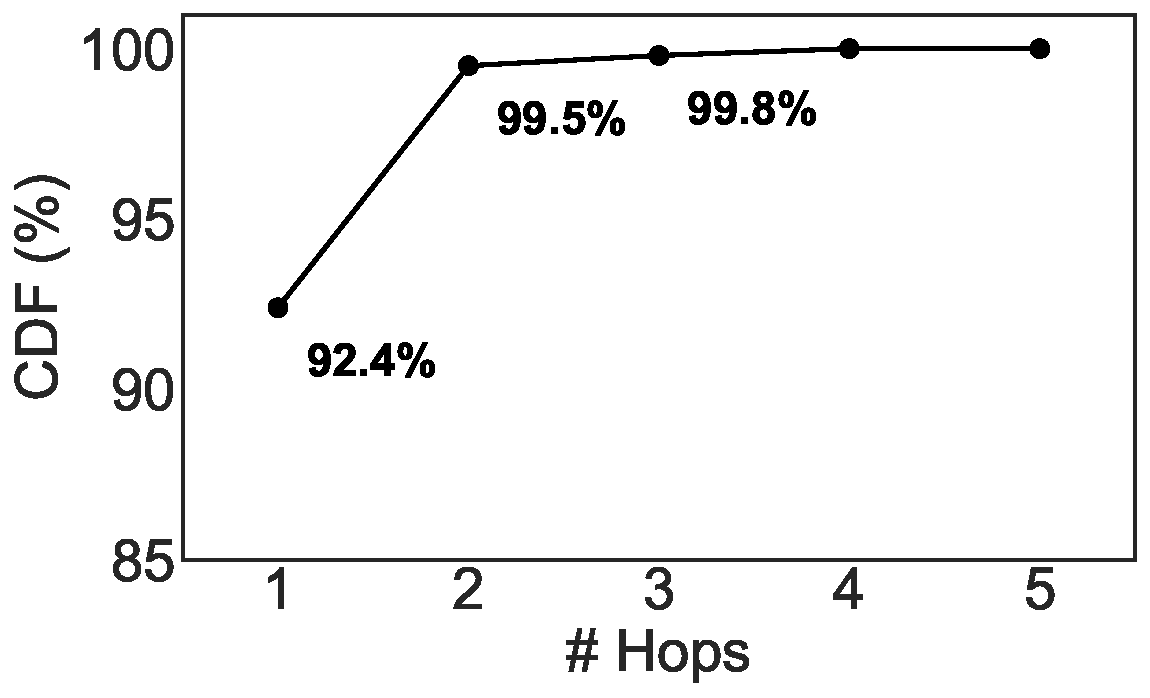
\includegraphics[width=0.35\textwidth]{figures/nonrpkicoverage.pdf}
    \caption{CDF of non-RPKI ASes that have at least one RPKI-enabled neighbor within a given AS-level hops distance, across 79,327 ASes as of April 2026.} %the full CAIDA topology (April 2026, ~\cite{caida-dataset}) with RPKI labels from rpki-client~\cite{rpki-client}.}
    \label{fig:rpki_hop_coverage}
\end{figure}





\subsection{Challenges} 
\md{Recent studies~\cite{saad2022routechain, chen2020isrchain} have explored blockchain-based enhancement for the BGP security infrastructure, motivated by its decentralized trust model, tamper-resistance, and ability to provide verifiable provenance of routing information. However, they fail to provide a reliable audit trail due to the following shortcomings:}


\BfPara{Asymmetric Knowledge in BGP Environment} 
\md{Recent blockchain-based approaches lack topological alignment, assuming a symmetric, global view of routing knowledge across ASes via a shared blockchain state, which fails to reflect the localized and policy-driven nature of real-world BGP deployment, where routing knowledge is asymmetric and context-dependent, as demonstrated in Figure~\ref{fig:asymmetric_knowledge}. As shown, unlike current blockchain deploymnet, where all nodes observe a shared transaction pool, BGP observers possess unique, vantage-point-dependent views: an observer at one router may see an announcement that is invisible or different from another. Therefore, existing solutions unable to agree on multiple, equally valid but divergent routing views, leading to inconsistencies in how events are being recorded and interpreted, resulting in inaccurate or biased global assessments of AS behavior. Moreover, enforcing a globally synchronized state across distributed and symmetric observations requires all-to-all cross-node communication to reach consensus, incurring $O(n^2)$ communication overhead, which does not scale to the large structure of the global Internet with over 70,000 ASes.}

%Existing blockchain-based BGP solutions lack consensus algorithms designed for this asymmetric environment. They struggle to reconcile these conflicting yet valid perspectives into a single, unified behavioral assessment. Thus, we propose a scalable consensus framework required for distributed observers to agree on an AS's historical behavior across diverse vantage points.


\begin{figure}[t]
\centering
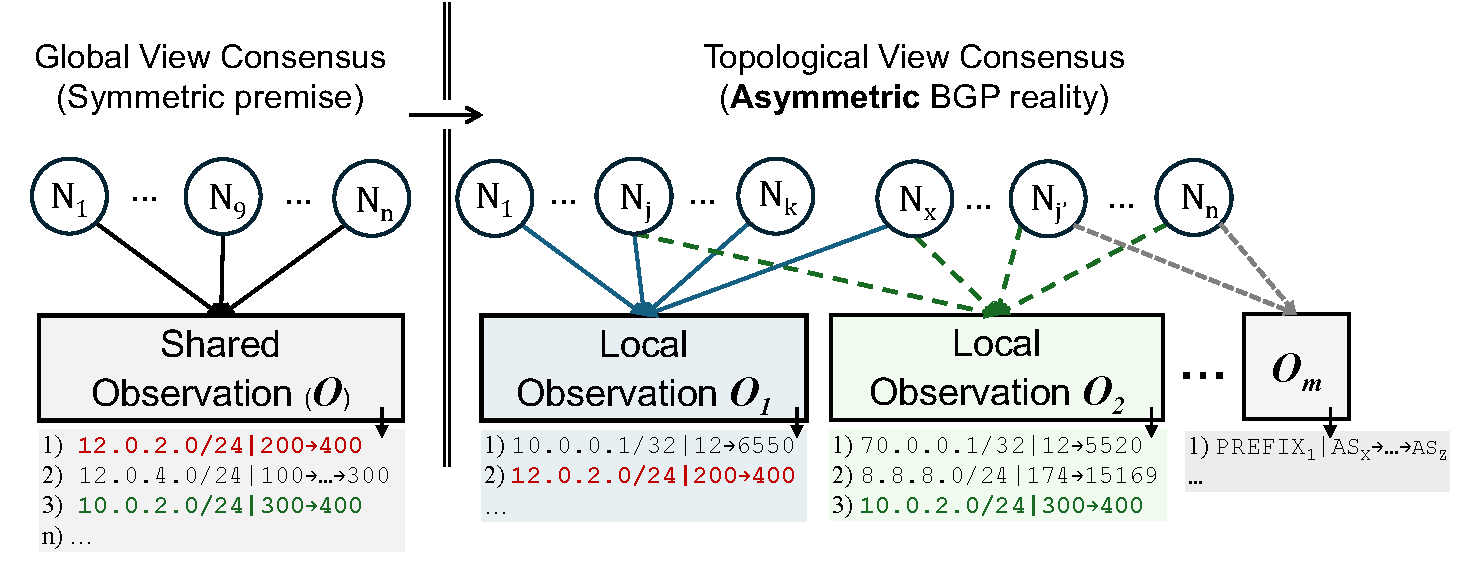
\includegraphics[width=0.5\textwidth]{figures/BGP-Asym.pdf}
\caption{Asymmetric knowledge in BGP: In a conventional blockchain, all nodes receive a uniform global observation $O$, whereas in a BGP environment, consensus inputs are heterogeneous local observations $O_i$, with each node seeing a partial view of routing events. 
% \os{Some notes: 1) Left side (Symmetric knowledge) is taking up more space for relatively a simple point. 2) Maybe highlight the features of announcements that are different across all ASes (to highlight asymmetry).}
}
\label{fig:asymmetric_knowledge}
\end{figure}



\BfPara{Rootless Identity and Event Integrity} 
\md{While blockchain offers a significant opportunity to extend decentralized trust, existing blockchain-based BGP security solutions are RPKI-agnostic, particularly during the critical selection and onboarding of nodes for consensus and validation. Prior work, RouteChain~\cite{saad2022routechain}, treats all nodes as equally trustworthy despite varying levels of routing competence and security commitment. They establish trust by randomly selecting nodes regardless of their RPKI status or routing credibility, creating a circular problem in which the system relies on unverified entities to validate routing information, potentially allowing malicious or misconfigured nodes to participate in consensus decisions that affect the integrity of the global routing security. 
This motivates a mechanism that is verifiable at onboarding and incentivized to behave honestly, enabling comprehensive surveillance of the entire BGP ecosystem.}


Through this multi-faceted approach, BGP-Sentry enhances routing security by complementing and strengthening the current RPKI ecosystem without requiring replacement or overhaul of existing infrastructure, allowing easy adoption across the Internet routing landscape.






\section{BGP-Sentry System Design}
\label{sec:system_threat_model}
In this section, we present the system and threat model, followed by an overview of BGP-Sentry.


\subsection{System Model}
\label{subsec:system_model}

\md{We define the system model for BGP-Sentry over the global inter-domain routing graph $G = (\mathcal{V}, \mathcal{E})$, where $\mathcal{V}$ is the set of Autonomous Systems ($\mathcal{AS}$). Our model builds on the partial deployment of RPKI as its foundation. We designate the subset of RPKI-compliant nodes $\mathcal{O} \subset \mathcal{V}$ as observers. These nodes leverage the global RPKI hierarchy as a root of trust, using cryptographically signed ROAs to verify prefix ownership. These observers also act as a bridge between the legacy BGP environment and our Blockchain security layer; they monitor updates from non-participating neighbors and execute a local detection pipeline to generate evidence for a distributed ledger $\mathcal{L}$. To maintain the integrity of this ledger, we assume a synchronous honest majority within the observer set $\mathcal{O}$, where at least a quorum $\tau$ of the observers involved in a validation task are non-adversarial and maintain consistent RPKI caches. 
Finally, observers leverage existing registries (e.g., RPKI repositories) of participating nodes to identify RPKI peers along a routing path as distributed witnesses for cross-verification before recording data in the immutable audit trail $\mathcal{L}$.}


\subsection{Threat Model}
\label{subsec:threat_model}
\md{We assume a Byzantine adversary~\cite{lamport2019byzantine} $\mathcal{A}$ representing a malicious or misconfigured Autonomous System (AS), including both non-RPKI participants and potentially compromised nodes within the RPKI observer set $\mathcal{O}$. We assume $\mathcal{A}$ is capable of injecting fraudulent routing information, such as prefix/sub-prefix hijacks~\cite{prefixHijacking}, bogon announcements~\cite{mao2003bgp}, to enable traffic interception, blackholing, or persistent network instability~\cite{butler2009survey}. We do not assume that RPKI compliance guarantees benign behavior in routing; an adversary $\mathcal{A}$ may still reside within $\mathcal{O}$ and engage in malicious BGP announcements. However, we assume that observations reported by RPKI-enabled nodes are honest, i.e., $\mathcal{A}$ does not falsify the data it contributes to the system. Under this assumption, $\mathcal{A}$ remains computationally bounded and cannot compromise standard cryptographic primitives (e.g., SHA-256), the RPKI root of trust, or the honest majority quorum in the blockchain model.}

% We assume RPKI compliance does not inherently guarantee benign behavior; thus, $\mathcal{A}$ may reside within $\mathcal{O}$, attempting to disrupt consensus via false observations or collusion to fork the ledger $\mathcal{L}$. 




\subsection{Overview of BGP-Sentry}
\label{subsec:defense_concept}

\md{We designed BGP-Sentry as a closed-loop framework that transforms transient BGP updates into a long-term audit trail for global visibility. As shown in Figure~\ref{fig:system-architecture}, while the existing RPKI infrastructure is limited to validating signed prefixes only from a portion of the network (i.e., RPKI nodes), BGP-Sentry leverages RPKI-compliant nodes as distributed observers to audit the behavior of the non-compliant ASes, building a unified visibility across the BGP network through trust expansion reflected in AS-level scoring. 
BGP-Sentry adapts PoP to the BGP setting rather than using it unchanged. First, identity is grounded not in general real-world identification, but in \emph{RPKI-verified AS identity} established during onboarding, so that a participant enters the consensus set only after proving control over its certificate chain and ROA-related cryptographic material. Second, the consensus object is not a financial transaction block, but a \emph{BGP observation} generated by an RPKI-enabled observer. 
At its core, the system operates as a four-stage cycle that progressively expands trust across the network:} 

%Third, because BGP exhibits \emph{asymmetric visibility}, where routing updates are observable only to topologically relevant neighbors and path-adjacent participants, validator selection must also follow routing visibility rather than global randomization. Accordingly, TrustChain employs a \emph{Data Plane-aware Proof-of-Population (DP-PoP)} model, in which observers seek endorsements only from RPKI-enabled peers with meaningful vantage points over the event, and record the observation once it accumulates the quorum threshold $\tau$. 
%As a result, TrustChain preserves the main advantage of PoP, identity-bound, population-backed, low-cost signature consensus, while avoiding blind voting and reducing unnecessary communication overhead. The blockchain, therefore, functions not only as a decentralized registry, but also as a \emph{behavioral attestation layer} that transforms transient routing observations into persistent, verifiable, and consensus-backed evidence, enabling longitudinal trust scoring and active security enforcement against both RPKI-participating and non-participating networks.


\md{\noindent\circled{1} \textbf{RPKI-enabled Collaborative Observation:} The workflow begins when RPKI-compliant observers receive BGP announcements from their peer ASes. Unlike legacy frameworks that generate isolated local alerts, BGP-Sentry leverages these nodes as distributed validators. That is, when it receives an announcement, it initiates a validation process to evaluate the observed event, preventing potential malicious activity (e.g., prefix hijack). This way, we elevate the event from a local observation to a collaborative inquiry. Because BGP exhibits \emph{asymmetric visibility}, where routing updates are observable only to topologically relevant neighbors and path-adjacent participants, BGP-sentry employs a \emph{Data Plane-aware Proof-of-Population (DP-PoP)} model, in which observers seek endorsements only from RPKI-enabled peers with meaningful vantage points over the event.}

\md{\noindent\circled{2} \textbf{PoP-verified Ledger Commitment:} To prevent false positives or malicious reporting by a compromised observer, BGP-Sentry employs a Proof-of-Population (PoP) consensus mechanism. The observer coordinates with a quorum $\tau$ of peers identified via the routing path to cross-verify the event. An event is committed to the ledger once it meets the required consensus threshold. This process ensures that all announcements are mathematically verifiable, grounding the network's events in a collective truth rather than separated claims.}

\md{\noindent\circled{3} \textbf{Immutable Forensic Audit Trail:} Once an event is validated, it is recorded in the immutable ledger $\mathcal{L}$, a persistent, cryptographically verifiable audit trail. This enables real-time validation and post-hoc analysis of AS behavior, allowing operators to enforce strict behavioral policies, reconstruct its evolution, and detect complex coordinated attacks that are invisible to single-node.}

\md{\noindent\circled{4} \textbf{Dynamic Trust Quantification and Security Enforcement:} The system closes the loop by translating historical evidence into active defense. BGP-Sentry maintains a Dynamic Trust Score $S$ for every non-RPKI and RPKI participants, initialized at a neutral baseline and adjusted based on verified behavior recorded in $\mathcal{L}$. When an AS's score falls below a critical threshold $\mathcal{T}$, the ledger propagates a ``malicious'' state across the consortium. Using this, participating routers trigger trust-based filtering, isolating an untrusted party by restricting its activity. This ensures an AS's past behavior directly dictates its validity, forming a self-reinforcing deterrent against BGP routing threats.}


\begin{figure}[t]
\centering
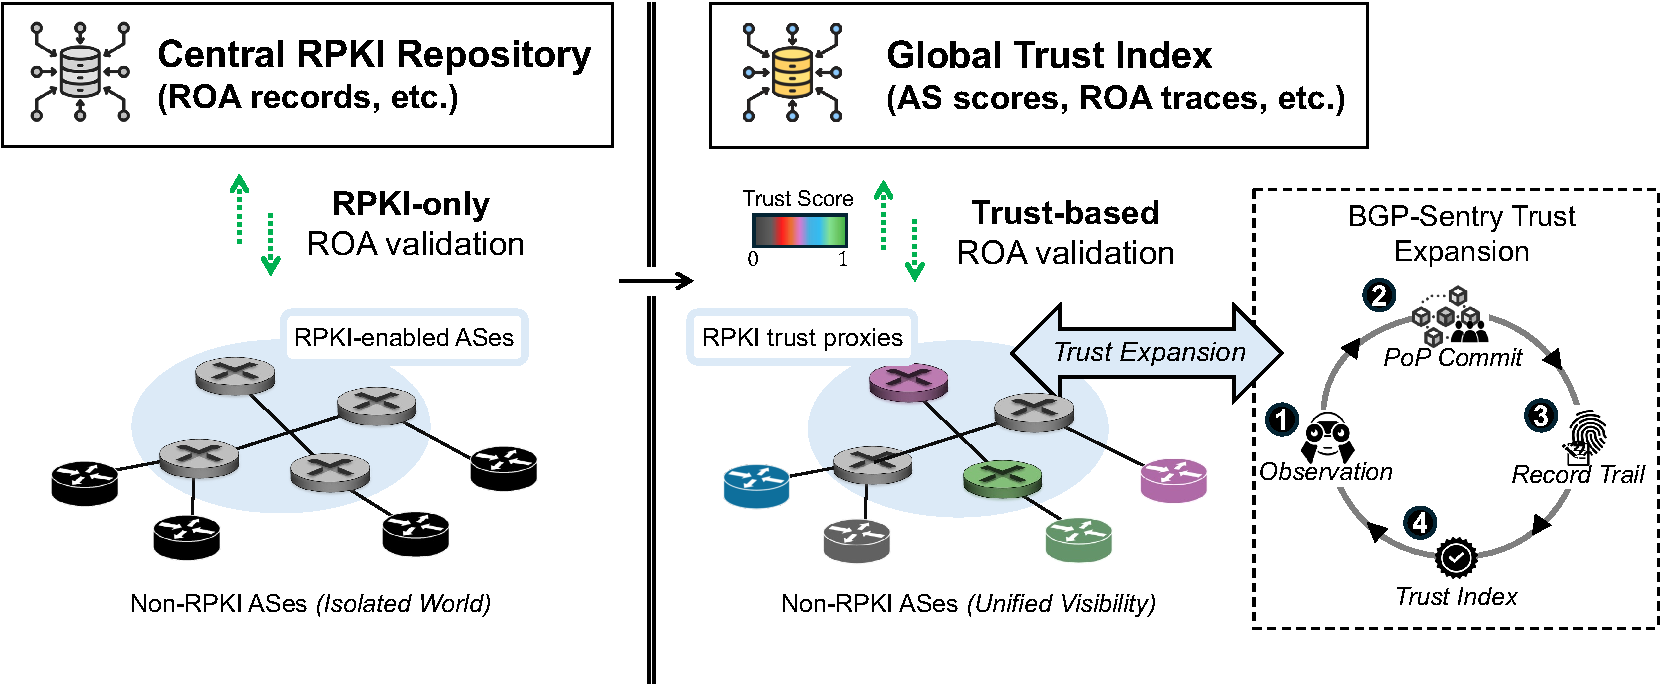
\includegraphics[width=0.5\textwidth]{figures/system.pdf}
\caption{Comparison of legacy RPKI-only validation (Left) with BGP-Sentry's unified observability (Right). While centralized RPKI leaves non-RPKI networks as unverified blind spots, BGP-Sentry employs a trust-expanded approach for universal visibility and trust-based ROA validation.
}
\label{fig:system-architecture}
\end{figure}



% \md{\textbf{[Mehdi] @Anik} The assumption about RPKI node behavior and the scoring mechanism is vague: 1) on one hand, we are assuming that RPKI nodes can also behave maliciously (which is possible due to misconfiguration or compromise cases), 2) on the other hand, we are only scoring the non-RPKI, then the question is what happens to the RPKI node in the scoring system?}






\section{Data Plane-aware Blockchain Design}
\label{sec:architecture}

This section details the core components that realize the system model and the threat model defined above. Figure~\ref{fig:system-architecture} illustrates the transformation from RPKI-only binary validation to full behavioral trust coverage.

\subsection{\rj{Onboarding: Bridging RPKI and Ledger Trust}}

\md{BGP-Sentry resolves the trust gap between the centralized RPKI hierarchy and the decentralized blockchain periphery by treating RPKI certificates as a root of identity. While RPKI provides cryptographic proof of prefix ownership, it lacks a native mechanism to bridge this authority into distributed ledger systems. Consequently, existing blockchain-based approaches often rely on unverified participants during onboarding, introducing Sybil vulnerabilities~\cite{saad2022routechain}. To address this, we implement an integrated trust model that anchors blockchain identities to RPKI resources through a challenge-response mechanism. This process creates a Sybil barrier, ensuring that every observer in the PoP consensus is cryptographically bound to physical network resources. The RPKI-anchored onboarding protocol is detailed in Figure~\ref{fig:onboarding}.}

\md{First, a candidate AS initiates participation by submitting its X.509 certificate chain and associated ROAs (\textit{Step 1}). Current validators first perform a structural check against RIR trust anchors to ensure the certificate is valid and unrevoked (\textit{Step 2}). This step confirms that the candidate possesses legitimate cryptographic standing within the global RPKI hierarchy. Next, to prevent identity spoofing, where an attacker presents a stolen certificate, the system issues an ROA key challenge (\textit{Step 3}). The candidate must provide a signed proof of resource ownership (\textit{Step 4}) using the private key associated with its RPKI certificate. This step prevents an adversary from spinning up multiple phantom identities without corresponding RIR-allocated prefixes.
Once the identity is anchored, existing members verify the proof and conduct a quorum-based vote to finalize admission (\textit{Steps 5-7}). Through this process, BGP-Sentry transforms RPKI-enabled ASes into Trust Proxies to enable previously opaque entities under a unified behavioral monitoring framework. 
}

% \rj{BGP-Sentry resolves the fundamental trust disconnect between the centralized RPKI hierarchy and the unverified, decentralized Internet periphery.While RPKI provides with cryptographic trust of IP prefix ownership, it doesn't have the feature to directly onboard verified  ASes into the distributed blockchain model. As a result existing blockchain based approaches rely on unverified participant during the on-boarding which introduces critical vulnerability or adversarial parties in the consensus process \cite{saad2022routechain}.
% To address this issue, we establish an \textit{integrated trust} model that extends cryptographic accountability to the data plane by requiring the candidate AS to prove the possession of a RPKI certificate resources through a challenge repose mechanism. This verified admission provides a strong Sybil resistance which is the key building block of PoP consensus mechanism. An overview of the RPKI-anchored on-boarding protocol steps are shown in the sequence diagram Figure~\ref{fig:onboarding}.}

% \rj{As shown, the protocol creates a cryptographic ``Sybil barrier'' to ensure ledger integrity. A candidate AS initiates participation by submitting its X.509 certificate chain and associated ROAs (Step 1). Validators perform a two-stage verification: first, validating the certificate against RIR trust anchors (Step 2), and second, issuing a ROA key challenge (Step 3). By requiring a signed proof of resource ownership (Step 4), the system ensures that the blockchain identity is permanently and cryptographically bound to the candidate's actual RPKI resources. Once this identity is anchored, existing members verify the proof and vote via a quorum-based admission process (Steps 5-7). This mechanism ensures that while the ledger is distributed, its root of trust remains centralized and verifiable, effectively fixing the ``blind spot'' of unverified non-RPKI entities by bringing them under a unified behavioral scoring framework managed by verified observers.}

% \textbf{@Anik}: Emphasize and discuss prior works RPKI+blockchain \textbf{[Cite]},  why this is critical issue. Also, explain more technical issues in realizing a secure RPKI-anchored onboarding process in the following, with steps 1-3. \textbf{@Mehdi}: Cross-check technical correctness for Anik's description.
\begin{figure}[t]
\centering
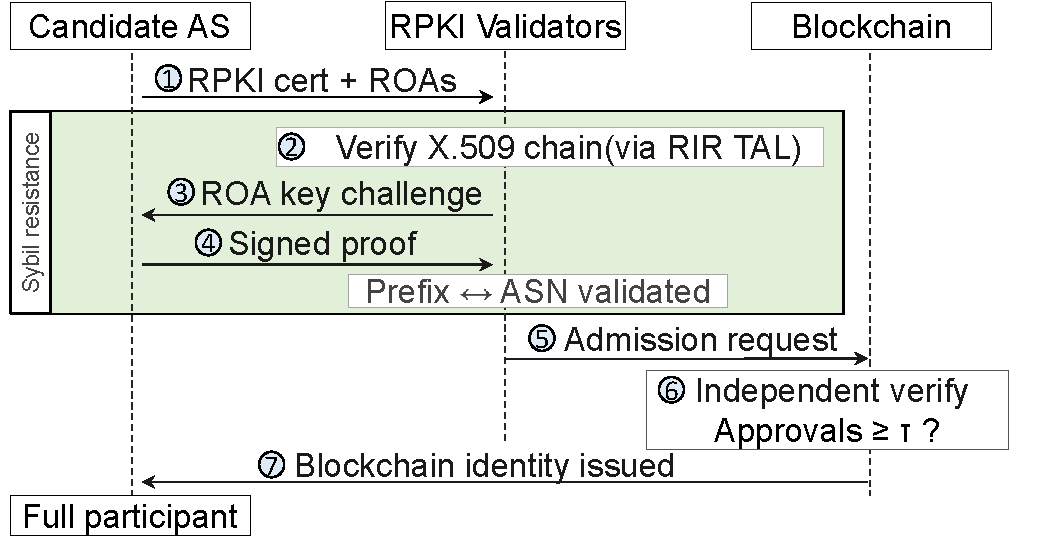
\includegraphics[width=0.4\textwidth]{figures/rpki_onboarding.pdf}
\caption{RPKI-verified onboarding protocol (sequence diagram). The candidate AS submits its RPKI certificate chain (step~1). Validators verify the X.509 chain against RIR trust anchors (step~2), then challenge the candidate to prove ROA key ownership (steps 3--4). This cryptographic verification forms the Sybil barrier: without a legitimate RPKI certificate, no entity can pass steps 2--4. Upon successful verification, validators broadcast an admission request to the consortium (step~5), where members independently verify and vote (step~6). If the quorum threshold $\tau$ is met, a blockchain identity cryptographically bound to the candidate's RPKI resources is issued (step~7), and the node joins as a full consensus participant.}
\label{fig:onboarding}
\end{figure}

% \begin{figure}[t]
% \centering
% 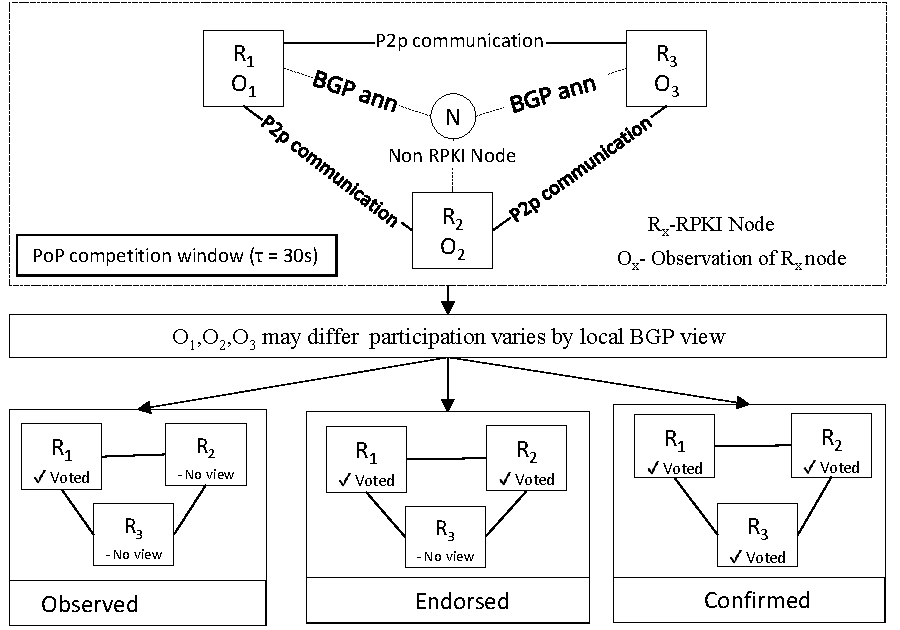
\includegraphics[width=1\columnwidth]{figures/pop.pdf}
% \caption{PoP consensus workflow and blockchain recording. The process illustrates the \textit{topological scoping} principle: the consensus boundary is mathematically constrained to the announcement path (observers $R_1, R_2, R_3$). This ensures that only nodes with a direct data-plane vantage point, the only entities capable of providing ground-truth verification, can participate in the PoP process, thereby eliminating ``blind-voting'' noise and reducing communication complexity from $O(N)$ to $O(k)$. The zoomed block $B_k$ details the on-chain record, including the verified BGP observation, trust scores, and PoP signatures. \rj{\textbf{@Anik@Mehdi}: This figure must demonstrate a \textbf{Data Plane-aware} and \textbf{Topological Scoping} concept, to justify the hop-limited-based consensus design for PoP customization. }}
% \label{fig:pop-consensus-workflow-1col}
% \end{figure}


\begin{figure}[t]
\centering
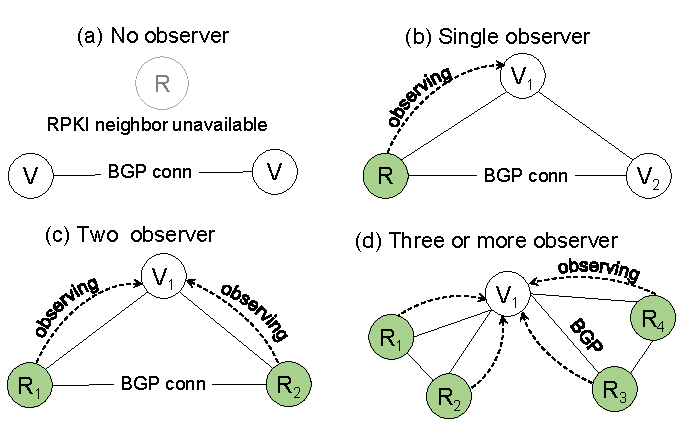
\includegraphics[width=0.4\textwidth]{figures/observer_coverage.pdf}
\caption{Observer coverage scenarios. (a)~No RPKI neighbor: no blockchain record (0\% in CAIDA data). (b)~Single observer: all behavior recorded, low confidence. (c)~Dual observers: cross-validated evidence, medium confidence. (d)~3+ observers: PoP consensus enables high-confidence verdicts and trust promotion. 
\os{For this figure: maybe follow same covention as well, grey color for nodes that are not trusted. Ri nodes to be filled with green color. For part (a), the cross on R node conveys a different message at first glance, as if the R node has been ousted by the network. With color scale, I believe the idea could be clearer.}
}
\label{fig:observer_scenarios}
\end{figure}

\subsection{\rj{Consensus: Data Plane-aware Proof of Population}}
\md{Unlike conventional blockchains, where participants share a global mempool, BGP monitoring yields fundamentally asymmetric observations. An AS may announce divergent routes to different neighbors due to local policy or poisoning attacks, meaning an event visible to one node may be topologically obscured from others. Consequently, consensus in BGP-Sentry must first establish the veracity of an observation before its commitment.}

% \rj{Unlike conventional blockchains, where all participants share a global view of pending transactions from a memory pool, BGP monitoring produces fundamentally asymmetric observations: each RPKI observer sees only the announcements that traverse its own network position, and an AS may announce different routes to different neighbors based on local policy, maintenance, or congestion management. This asymmetry means that a routing event observed by one node may be invisible to others, or may appear differently depending on the observer's topological vantage point. In some cases, an announcement may be witnessed by only a few observers-a scenario that can also arise from sophisticated targeted attacks. Reliable behavioral assessment, therefore, requires aggregating these partial, potentially conflicting views into a coherent longitudinal record, from which the behavior of an unverified AS can be systematically determined. With this challenge in mind, we design the consensus process as follows.}


\subsubsection{Consensus Protocol Design}
\md{In traditional Proof-of-Work (PoW) or Proof-of-Stake (PoS) systems, consensus is primarily a problem of total ordering to prevent double-spending~\cite{nakamoto2008bitcoin}. However, the requirement for strict global synchronization introduces significant latency and throughput bottlenecks.
In contrast, BGP updates for different prefix–origin pairs are largely independent. Leveraging this fact, we relax BGP-Sentry's requirement for a strict global ordering and instead prioritize concurrent log integrity. This design enables scalable processing across independent update streams and eliminates the need for a ``competition for the next block''. Instead, we adopt observational corroboration, rewarding nodes based on their topological vantage points and knowledge sharing.}

\md{When an RPKI observer $\mathcal{O}_i$ receives an announcement from a non-RPKI neighbor, it performs the pipeline in Algorithm~\ref{alg:integrated_consensus}. It begins with redundant update filtering and the generation of a signed transaction, followed by a Path-Aware Discovery to broadcast vote requests to topologically relevant peers (lines 1-6). Each peer independently validates the observation against its local RIB/FIB state and returns a cryptographic endorsement if the event is confirmed. The first node to accumulate the required endorsement threshold (e.g., $\tau \geq 3$) within the competition window (lines 7-13) commits the transaction to the ledger (lines 14-15). This ensures that recorded observations are backed by multiple independent vantage points, preventing a single Byzantine participant from fabricating a consensus agreement.}

\md{Upon successful commitment, the system triggers the pipeline in Algorithm~\ref{alg:integrated_scoring}. This stage executes multi-vantage point attack detection and applies quorum-based classification to update trust scores and participation credits to enable a security assessment bound to the Integrated Trust model.}

% \rj{In any conventional blockchain, a competition mechanism determines which node will append the next block: Proof-of-Work rewards the fastest computationally \cite{nakamoto2008bitcoin}, while Proof-of-Stake selects validators in proportion to their locked capital \cite{buterin2014ethereum}. Both approaches assume a shared transaction pool visible to all participants, reducing consensus to a problem of ordering. By contrast, BGP-Sentry operates on a fundamentally different premise: because routing observations are asymmetric and no shared mempool exists, consensus must first establish the validity of an observation before recording it. The competition in our Proof-of-Population \cite{} mechanism is therefore based on observational corroboration rather than computation or economic stake. }


%  \rj{When an RPKI observer processes a BGP announcement from a non-RPKI neighbor, it executes the integrated pipeline formalized in Algorithm~\ref{alg:integrated_consensus}. This involves creating a signed transaction and broadcasting a vote request to topologically relevant peers discovered via path-aware discovery (lines 1-6). Each peer independently validates the observation against its local knowledge base, returning an endorsement if it can corroborate the event. The first node to accumulate the required endorsement threshold ($\tau \geq 3$) within the competition window (lines 7-13) commits the transaction to the blockchain (lines 14-15). This ensures recorded observations are backed by multiple independent vantage points, preventing any single participant from fabricating agreement.}



% \rj{We formalize the BGP-Sentry framework through two integrated algorithms. Algorithm~\ref{alg:integrated_consensus} governs the end-to-end \textit{Data Plane-Aware Consensus}, which handles redundant update filtering, targeted observer discovery via topological scoping, and time-bounded signature collection. Upon successful commitment to the ledger, the system triggers the \textit{Behavioral Attribution} pipeline, as shown in Algorithm~\ref{alg:integrated_scoring}. This second stage executes multi-vantage point attack detection, applies quorum-based classification, and updates trust scores and participation credits. This two-stage architecture ensures that every recorded observation is not only corroborated by peers but also carries a corresponding security assessment bound to the Integrated Trust model.}


% \begin{algorithm}[t]
% \caption{Integrated Data Plane-Aware Consensus}
% \label{alg:integrated_consensus}
% \begin{algorithmic}[1]
% \Statex \textbf{Input:} BGP Event $e$, Local Node $N_i$, Threshold $\tau$, AS-Path $\mathcal{P}$
% \Statex \textbf{Output:} Transaction $TX$ committed to Ledger $\mathcal{L}$

% \Statex \textit{// Phase 1: Filtering \& Discovery (Topological Scoping)}

% \State $ID_{e} \gets (\mathit{prefix}, \mathit{originAS})$
% \If{$ID_{e} \in \mathit{Cache}$ \textbf{or} $\mathit{age}(ID_e) < T_{\mathit{sample}}$} \Return $\bot$ \EndIf

% \State $\mathcal{V} \gets \{N_j \mid N_j \in \mathcal{N}_k(\mathcal{P}) \cap \text{RPKI-Set}\}$ \label{line:discovery}

% \If{$|\mathcal{V}| < \tau$} $\mathcal{V} \gets \mathcal{V} \cup \text{Sample}(\text{Registry}, \tau)$ \EndIf

% \Statex \textit{// Phase 2: Time-Bounded Corroboration}
% \State $TX \gets \text{Sign}(e, SK_i)$, $\mathcal{S} \gets \emptyset$, $t_0 \gets \text{clock}()$
% \State \textbf{broadcast} $TX$ to $N_j \in \mathcal{V}, \forall_j$
% \While{$\text{clock}() - t_0 < T_{\mathit{win}}$ \textbf{and} $|\mathcal{S}| < \tau$}
%     \State $s_j \gets \text{ReceiveSignature}(N_j)$
%     \If{$\text{Verify}(s_j, N_j)$ \textbf{and} $N_j \in \mathcal{V}$}
%         \State $\mathcal{S} \gets \mathcal{S} \cup \{s_j\}$
%     \EndIf
% \EndWhile

% \Statex \textit{// Phase 3: Commitment \& Graduation}
% \State $TX_\mathit{status} \gets (|\mathcal{S}| \geq \tau) ? \text{\texttt{CONFIRMED}} : \text{\texttt{OBSERVED}}$
% \State $\text{CommitToLedger}(TX, \mathcal{S})$
% \State \Return $TX$
% \end{algorithmic}
% \end{algorithm}

% \begin{algorithm}[t]
% \caption{Integrated Trust Scoring and Incentives}
% \label{alg:integrated_scoring}
% \begin{algorithmic}[1]
% \Statex \textbf{Input:} Transaction $TX$, Trust Table $\mathcal{T}$, Ledger $\mathcal{L}$
% \Statex \textbf{Output:} Updated Scores and Participation Credits

% \Statex \textit{// Phase 1: Multi-Vantage Point Detection}

% \State $\mathit{type} \gets \text{Classify}(TX)$, $\mathit{origin} \gets TX.\mathit{originAS}$
% %\State $\mathit{alerts} \gets \text{Detect}(TX)$
% %\If{$\mathit{alerts} = \emptyset$}
% \If{$\mathit{type} = \text{\texttt{LEGITIMATE}}$}
%     \State $\mathcal{T}[\mathit{origin}].\mathit{count} \gets \mathcal{T}[\mathit{origin}].\mathit{count} + 1$
%     \State \textbf{if} $(\mathit{count} \pmod{100} = 0)$ \textbf{then}\\
%     $\mathcal{T}[\mathit{origin}].\mathit{score} \gets \mathcal{T}[\mathit{origin}].\mathit{score} + 1$
%     \State \Return
% \EndIf

% \Statex \textit{// Phase 2: Reactive Penalty \& Observer Rewards}
% \State $\mathit{quorum} \gets \text{MajorityVote}(\mathit{alerts})$
% \If{$\mathit{quorum} = \text{Valid}$}
%     \State $P \gets \text{CalcPenalty}(\mathit{type}, \mathit{history})$
%     \State $\mathcal{T}[\mathit{origin}].\mathit{score} \gets \mathcal{T}[\mathit{origin}].\mathit{score} - P$
%     \State $\mathcal{L}[\mathit{observers}] \gets \mathcal{L}[\mathit{observers}] + \text{Credits}_{\mathit{reward}}$
% \Else
%     \State $\mathcal{L}[\mathit{proposer}] \gets \mathcal{L}[\mathit{proposer}] - \text{Penalty}_{\mathit{false\_report}}$
% \EndIf
% \end{algorithmic}
% \end{algorithm}

\begin{algorithm}[t]
{
\caption{Integrated Data Plane-Aware Consensus}
\label{alg:integrated_consensus}
\KwIn{
BGP Event $e$, Local Node $N_i$, Threshold $\tau$, AS-Path $\mathcal{P}$
}

$ID_{e} \gets (\mathit{prefix}, \mathit{originAS})$\;
\If{$ID_{e} \in \mathit{Cache}$ $\vee$ $\mathit{age}(ID_e) < T_{\mathit{sample}}$}{
    \Return $\bot$; \Comment{Filtering Recent events}
}

% Phase 1: Discovery
\tcp{Path-Aware Discovery}
$\mathcal{V} \gets \{N_j \mid N_j \in \mathcal{N}_k(\mathcal{P}) \cap \text{RPKI-Set}\}$\;
\If{$|\mathcal{V}| < \tau$}{
    $\mathcal{V} \gets \mathcal{V} \cup \text{Sample}(\text{Registry}, \tau)$; \Comment{Sampling}
}

% Phase 2: Corroboration
\tcp{Time-Bounded Corroboration}
$TX \gets \text{Sign}(e, SK_i)$, $\mathcal{S} \gets \emptyset$, $t_0 \gets \text{clock}()$\;
\textbf{broadcast} $TX$ to all $N_j \in \mathcal{V}$\;

\While{$\text{clock}() - t_0 < T_{\mathit{win}}$  $ \wedge$ $|\mathcal{S}| < \tau$}{
    $s_j \gets \text{ReceiveSignature}(N_j)$\;
    \If{$\text{Verify}(s_j, N_j) \wedge N_j \in \mathcal{V}$}{
        $\mathcal{S} \gets \mathcal{S} \cup \{s_j\}$\;
    }
}

% Phase 3: Commitment
\tcp{State Graduation and Ledger Entry}
% $TX_\mathit{status} \gets (|\mathcal{S}| \geq \tau) ? \text{\texttt{CONFIRMED}} : \text{\texttt{OBSERVED}}$\;

$TX_{\mathit{status}} \gets 
\text{\texttt{CONFIRMED}} \;\text{if}\; |\mathcal{S}| \geq \tau 
\;\text{else}\; \text{\texttt{OBSERVED}}$\;
$\text{CommitToLedger}(TX, \mathcal{S})$\;

\Return $TX$\;
}
\end{algorithm}



\begin{algorithm}[t]
{
\SetKwIF{If}{ElseIf}{Else}{if}{}{else if}{else}{end if}
\caption{Integrated Trust Scoring and Incentives}
\label{alg:integrated_scoring}
\KwIn{
Transaction $TX$, Trust Table $\mathcal{T}$, Ledger $\mathcal{L}$
}

$\mathit{type} \gets \text{Classify}(TX)$, $\mathcal{A}_{\mathit{org}} \gets TX.\mathit{originAS}$\;

% Phase 1: Adaptive Recovery
%\tcp{Adaptive Recovery}
\If{$\mathit{type} = \text{\texttt{LEGITIMATE}}$ \hspace{2mm} \textnormal{\textbf{then}}}{ 
    $\mathcal{T}[\mathcal{A}_{\mathit{org}}].\mathit{count} \gets \mathcal{T}[\mathcal{A}_{\mathit{org}}].\mathit{count} + 1$\;
    \If{$\mathit{count} \pmod{100} = 0$}{
        $\mathcal{T}[\mathcal{A}_{\mathit{org}}].\mathit{score} \gets \mathcal{T}[\mathcal{A}_{\mathit{org}}].\mathit{score} + 1$\;
    }
}


% Phase 2: Reactive Enforcement
%\tcp{Reactive Enforcement}
$\mathit{quorum} \gets \text{MajorityVote}(TX)$\;
\eIf{$\mathit{quorum} = \text{Valid}$ \hspace{2mm} \textnormal{\textbf{then}} \Comment{Penalty \& Reward}}{
    $P \gets P_{base} \times S_{weight} \times R_{factor}$; \Comment{Eq. 1}\\ 
    $\mathcal{T}[\mathcal{A}_{\mathit{org}}].\mathit{score} \gets \mathcal{T}[\mathcal{A}_{\mathit{org}}].\mathit{score} - P$\;
    $\mathcal{L}[\mathit{observers}] \gets \mathcal{L}[\mathit{observers}] + R_{\text{honest}}$\;
}{
    $\mathcal{L}[\mathit{proposer}] \gets \mathcal{L}[\mathit{proposer}] - P_{\text{misreport}}$\;
}

\Return{$\mathcal{T}, \mathcal{L}$}\;
}
\end{algorithm}


\subsubsection{Path-Aware Discovery} 

\md{Recall that in the BGP decentralized model, BGP announcements are fundamentally asymmetric knowledge, unlike financial transactions in a global mempool; a routing update is only visible to nodes along its propagation path. A naive consensus approach would require broadcasting every update to all $N$ participants in the network. However, such a global model incurs unacceptable computational overhead and, more critically, introduces the ``Blind Voter'' problem, where nodes lacking a direct topological vantage point are forced to vote based on second-hand information, creating $O(N)$ false-positive risks.}

\textcolor{red}{\textbf{@Anik: please update and extend this part with the new path-discovery mechanism.}}

To address this, BGP-Sentry employs a Path-Aware Discovery mechanism. Rather than querying the entire network, nodes participate in a continuous knowledge buildup. By analyzing the audit trail of previous transactions, observers learn and cache the set of peers that consistently share a common observation pool for specific prefixes. This allows the system to dynamically map the set of relevant observers for any given transaction.

The feasibility of this discovery process is grounded in the real-world topology of the Internet. Figure~\ref{fig:observer_scenarios} illustrates four coverage scenarios identified in our analysis of the CAIDA dataset~\cite{caida-dataset}, which indicate the achievable consensus depth for these discovered sets. These scenarios are defined by the density of RPKI-enabled observers within the immediate first-hop ($k=1$) of an AS node:

(a) Isolated: No RPKI neighbors. In our analysis, we found that this scenario does not occur, ensuring that every AS is adjacent to at least one potential observer. (b) Single-Witness: The majority of ASes (67--85\%) fall under this category. While extending the observer into two immediately would reduce the impact, we handle the introduced uncertainty through a post-hoc Single-Witness Accumulation analysis (Section~\ref{subsec:posthoc_building_blocks}). (c) and (d) Multi-Vantage: These scenarios enable full PoP Consensus, providing cross-validated evidence and progressively tighter confidence bounds ($C_{conf} = 1 - 1/\sqrt{N_{obs} + 1}$).

% \md{By constraining the validator set to immediate, path-adjacent observers ($k=1$), BGP-Sentry ensures that every transaction is backed by a direct, local data-plane observation. This ensures the audit trail's integrity is directly proportional to the physical propagation of the BGP announcement itself, effectively eliminating ``Blind Voter'' noise from distant, non-witnessing nodes.}

% \rj{The effectiveness of this hop-limited design is verified by the reduction of the ``Blind Voter'' noise. In a global consensus model, nodes without a topological vantage point would be forced to vote based on second-hand information, introducing $O(N)$ false-positive risks. By constraining the validator set to path-adjacent observers, BGP-Sentry ensures that every vote is backed by a local data-plane observation. This results in a ``path-invariant'' consensus where the audit trail's integrity is directly proportional to the physical propagation of the BGP announcement itself.}






\subsection{\rj{Trust Orchestration: Integrated Behavioral Incentives}}

\md{To operationalize the \textit{integrated trust} established during onboarding, BGP-Sentry employs a dual-engine framework that converts transient observations into a longitudinal accountability record.}

% \rj{To operationalize the "integrated trust" established during onboarding, BGP-Sentry employs a dual-engine framework that converts transient observations into a longitudinal accountability record. This framework bridges gaps between RPKI’s static identity and the dynamic reality of BGP behavior.}

\BfPara{Reactive Trust via Immediate Penalty Enforcement} 
\md{The Reactive Trust design provides sub-second responses to confirmed violations. When an attack (e.g., prefix hijacking or bogon injection) reaches the PoP consensus threshold $\tau$, an immediate penalty is applied:
\begin{equation}
Penalty = P_{base} \times S_{weight} \times R_{factor}
\end{equation}
where $P_{base}$ is specific to the attack type (e.g., $P_{prefix}=20$, $P_{bogon}=25$). This ensures that malicious actors face immediate routing deterrence, effectively ``turning off'' the trust extended by the RPKI root.}

\BfPara{Adaptive Trust via Behavioral Recovery and Rewards} 
\md{While penalties are rapid, trust is earned longitudinally. The Adaptive Trust Engine rewards sustained clean behavior, granting $+1$ trust point per 100 legitimate observations. This ensures that the system remains fair, allowing for recovery from accidental misconfigurations while remaining Byzantine-resilient against persistent attackers.}

% \rj{While penalties are immediate, trust is earned longitudinally. The Adaptive Trust Engine conducts periodic evaluations of an AS’s 30-day historical performance. This is the only mechanism for trust score improvement, rewarding sustained clean behavior with ``trust points'' (+1 per 100 clean observations). This dual-layer approach, combining rapid deterrence with a path to rehabilitation, ensures the system remains both secure and fair, incentivizing non-RPKI entities to maintain high behavioral standards to retain their routing privileges.}


 

\subsection{\rj{Audit Utility: Verification of Integrated Trust}} \label{subsec:posthoc_building_blocks}

\md{The blockchain ledger $\mathcal{L}$ serves as the definitive source of truth for longitudinal forensic accountability, enabling three core analytical capabilities:}

% \rj{Beyond real-time enforcement, the \textit{integrated trust} model is operationalized through the longitudinal rigor of the blockchain ledger $L$. By synthesizing multi-vantage point observations into a tamper-evident audit trail, we enable a suite of \textit{post-hoc forensic analyses} that convert transient BGP updates into verifiable behavioral intelligence. These retrospective capabilities transcend the limitations of point-in-time monitoring, allowing the system to mathematically verify behavioral evolution, identify coordinated adversarial campaigns, and audit observer integrity. By bridging centralized RPKI authority with decentralized forensic enforcement, the audit trail serves as the definitive source of truth for long-term data plane accountability.}

\BfPara{Correlative Stability Analysis} 
\md{BGP-Sentry identifies route flapping by correlating oscillation signals across topologically diverse observers. By distinguishing systemic attacks from localized convergence artifacts, we ensure that transient noise does not unfairly degrade an AS's long-term reputation.}
% \rj{BGP-Sentry overcomes the false-positive limitations of single-observer flapping detection by correlating oscillation signals across topologically diverse observers. By identifying repeated announcements for the same $(prefix, origin)$ within overlapping windows, the system distinguishes systemic attacks from localized convergence artifacts. This transition from real-time capture to cross-observer validation ensures that transient noise is filtered before impacting long-term reputation.}

\BfPara{Single-Witness Accumulation} 
\md{Reflecting the reality that 67--85\% of ASes currently fall under single-observer scenarios (Scenario b), we record all observations regardless of initial consensus. While a single entry carries low confidence, the accumulation of independent reports over time delivers a composite certainty $C$:
\begin{equation}
C = 1 - (N_{obs} + 1)^{-1/2}
\end{equation}
This ensures that even in sparse deployments, localized observations aggregate into global certainties, effectively eliminating blind spots over time.}

% \rj{To ensure no behavior escapes accountability, the ledger records every observation regardless of its initial consensus status (Algorithm 1). While a \texttt{SINGLE\_WITNESS} entry carries low individual confidence, the longitudinal aggregation of independent reports for the same entity yields progressively higher composite certainty, defined as $C = 1 - (N_{obs} + 1)^{-1/2}$. This mechanism proves that a hop-limited consensus does not sacrifice security, as localized observations aggregate into global certainties over time.}

\BfPara{Adversarial Profiling and Integrity} 
\md{The audit trail enables detection of ``trust-score gaming'' (cyclical attack/recovery patterns) and coordinated multi-AS campaigns. Furthermore, we perform Observer Integrity Auditing, flagging validators whose voting patterns deviate significantly ($>2\sigma$) from the population mean, protecting the ledger from compromised or Byzantine RPKI observers.}

% \rj{The audit trail enables the detection of sophisticated adversarial strategies, such as coordinated multi-AS hijacks and ``trust-score gaming'' (cyclical attack/recovery patterns). By reconstructing the behavioral evolution of an AS, operators can identify anomalies invisible to per-event detection. Furthermore, the system performs \textit{Observer Integrity Auditing}, identifying statistical outliers whose detection records deviate significantly ($>2\sigma$) from the population means, allowing for the proactive adjustment of validator weights.}


\section{\rj{Implementation and Simulation}}
We implemented the BGP-Sentry in Rust(Stable 1.78) usig Tokio async runtime.The   implementation includes 7100 lines of code across 16 modules, organized into four architectural layers: observation, consensus,node management and simulation orchestration. An initial Python 3.10 prototype (13k LOC) validated the protocol
design; the Rust re-implementation was motivated by Python’s Global Interpreter Lock (GIL) bottleneck, which serializes all threads
onto a single core and caused consensus-timeout starvation at topology scales beyond 400 nodes.

\BfPara{Prototype Architecture}
The system is divided into four main modules. The BGP observation layer replays pre-recorded BGP announcement datasets and hosts five independent attack detectors, prefix
hijack, bogon injection, route flapping, route leak, and path poisoning, each operating as a stateless classification pipeline over incoming BGP UPDATE records. The blockchain and consensus stack implements a per-node block-lattice ledger with Tokio-based asynchronous P2P messaging, SHA-256 hash-chain
integrity, and the Data Plane-aware Proof-of-Population (PoP) consensus protocol, including transaction pooling, signature collection, and cross-chain synchronization. The node management layer instantiates and orchestrates the full set of virtual nodes,handling lifecycle events such as BGP announcement monitoring, transaction creation, vote solicitation, peer endorsement,
and knowledge-base maintenance. Finally, the simulation harness provides the experiment orchestrator: a synchronized wallclock that maps pre-recorded BGP timestamps to simulation
time, the end-to-end blockchain pipeline from observation to ledger commit, and post-hoc analysis, decoupling experimental control from protocol logic.



\BfPara{Simulation environment}
All experiments were conducted on a dual-socket Intel Xeon Platinum 8358 server (64 cores, 128 threads, 2.60\,GHz) with 1\,TB RAM running Ubuntu 22.04. The simulation relays the prerecorded BGP announcement to the   the full network of virtual blockchain nodes running a Tokio async runtime. Inter-node communication uses in-memory async message bus with guaranteed order delivery  replacing the tcp socket to enable large scale 5008 node simulation in a single machine. A shared global wall clock maps the BGP announcement timestamp to the wall clock, so that the observations are processed in time order.All consensus timeouts, de-duplication windows, and knowledge base expiry operate on a scaled simulation time, ensuring consistent protocol behavior independent of execution speed.

Nevertheless, the single machine simulation creates a resource bottleneck, where all the nodes are competing for the shared cpu cycle, memory bandwidth and the serialized message bus. In a production level deployment each node will have a dedicated infrastructure, alleviating this bottlenecks and improving the consensus commit rate. Result presented in the Section~\ref{sec:evaluation} should therefore be considered as lower bound of achievable throughput.

\BfPara{Dataset generation}
 Since there is no public dataset pairs BGP announcements with ground-truth attack labels at the scales we need, we build a synthetic dataset grounded in real measurement data, following common practice in BGP security evaluation~\cite{furuness2024bgpy}. We start from the CAIDA AS-relationships graph (April 2026 snapshot, 79K ASes)~\cite{caida-dataset} and carve out four regional transit backbones for AFRINIC, ARIN, and LACNIC, ranging from 904 to 5{,}008 ASes. The extraction targets transit ASes but also retains leaf ASes that connect to them; all RPKI-enabled ASes act as blockchain validators regardless of tier, while non-RPKI ASes participate only as observed edgenodes. RPKI labels come directly from the \texttt{rpki-client} VRP dump of April 2026 (all five RIR TALs), giving each topology its natural signing rate (49--68\%) without artificial normalization. Every AS gets one real IPv4 prefix: RPKI nodes draw theirs from VRP records, non-RPKI nodes from RouteViews~\cite{routeviews}.

The main simulation challenge is that BGPy~\cite{furuness2024bgpy} is event driven and assigns only symbolic timestamps (0 for victims, 1 for attackers), whereas our detectors rely on wall-clock sliding windows. We therefore add a Unix-epoch timestamp field to BGPy's \texttt{Announcement} class and layer on three timing models: (i)~a Poisson-arrival timeline that spreads legitimate announcements over a 12-hour window while placing attacks uniformly ; (ii)~per-hop convergence jitter drawn from a log-normal (median 5.5\,s, $\sigma{=}0.75$, clamped to $[1,20]$\,s) and accumulated along the AS-path~\cite{labovitz2001delayed}; and (iii)~withdrawal events for 10\% of prefixes, delayed by a log-normal (median 30\,s, clamped to $[10,180]$\,s). Each AS announces its prefix 2--4 times through Gao--Rexford valley-free propagation. We inject five attack types, namely prefix hijack, bogon injection, route flapping (5--9 oscillation cycles each), path poisoning, and route leak, at 2--3 events per type; path poisoning and route leak are crafted outside BGPy because it lacks native models for these vectors. A filter pass then drops prefixes longer than /24, caps observers per event at 20, and thins legitimate traffic to ${\approx}$0.005 events/sec/node (matching RIPE RIS 2022 steady-state rates). This per-node rate is held constant across all four topologies so that the total observation volume grows naturally with network size (222K at 904 ASes to 1.22M at 5{,}008), mirroring how real BGP traffic scales with the number of participating ASes. Final attack ratios is maintained under 0.5\%.



\section{Evaluation}

  \subsection{Experimental Setup}
  \label{sec:dataset}

We evaluate BGP-Sentry on the four regional datasets described in Section~VI. Table~\ref{tab:dataset_stats} summarizes topology and observation statistics. The four topologies span 904 to 5{,}008 ASes across three RIR regions with natural RPKI signing rates between 49\% and 68\%. Total observations grow from 7.6M to 177.7M as the topology scales, with the per-node event rate held constant. The three smaller topologies carry only legitimate traffic for scalability evaluation; the largest (LACNIC, 5{,}008 ASes) additionally includes five attack types for security evaluation.


\begin{table}[t]
  \caption{Regional dataset statistics. The three smaller topologies contain only legitimate traffic (scalability evaluation); LACNIC additionally includes attacks (security evaluation).}
  \label{tab:dataset_stats}
  \begin{threeparttable}
    \footnotesize
    \setlength{\tabcolsep}{4pt}
    \begin{tabular*}{\columnwidth}{l @{\extracolsep{\fill}} rrrr}
      \toprule
      \textbf{Metric} & \textbf{AFRI}\tnote{a} & \textbf{ARIN}\tnote{b} &
      \textbf{LA+AF}\tnote{c} & \textbf{LACNIC}\tnote{d} \\
      \midrule
      \textit{Topology} \\
      \quad Total ASes            & 904     & 2{,}030  & 3{,}152  & 5{,}008 \\
      \quad RPKI validators (\%)  & 49.2    & 67.5     & 61.2     & 53.3 \\
      \quad CP / Peer links       & 1.9K/4.8K & 4.9K/6.2K & 7.0K/17.3K & 10.9K/11.6K \\
      \quad Sim. duration          & 12\,h   & 12\,h    & 12\,h    & 12\,h \\
      \midrule
      \textit{Observations} \\
      \quad Total                 & 7.59M   & 41.9M    & 105.2M   & 177.7M \\
      \quad Legitimate (\%)       & 100     & 100      & 100      & 99.8 \\
      \quad Attack (\%)           & --      & --       & --       & 0.23 \\
      \midrule
      \multicolumn{5}{l}{\textit{Attack breakdown (LACNIC only)}} \\
      \quad Prefix Hijack         & -- & -- & -- & 22{,}001 \\
      \quad Bogon Injection       & -- & -- & -- & 59{,}042 \\
      \quad Route Flapping        & -- & -- & -- & 303{,}588 \\
      \quad Path Poisoning        & -- & -- & -- & 17{,}922 \\
      \quad Route Leak            & -- & -- & -- & 59 \\
      \bottomrule
    \end{tabular*}
    \begin{tablenotes}
      \footnotesize
      \item[a] AFRINIC transit + multihomed.
      \item[b] ARIN transit.
      \item[c] LACNIC + AFRINIC transit.
      \item[d] LACNIC 5+ customers, with attack injection.
    \end{tablenotes}
  \end{threeparttable}
\end{table}






% ─── B. Observation Completeness ───────────────────────────────────
\subsection{Observation Completeness}
\label{subsec:observation_completeness}

The first requirement for a blockchain-based audit trail is that no BGP observation is lost between ingestion and ledger commit. Table~\ref{tab:completeness} reports the observation pipeline across all four topologies. Each RPKI validator ingests announcements from the dataset, applies deduplication (skipping repeated prefix-origin pairs within a configurable window), and creates a blockchain transaction for every unique observation. Across all four topologies, every transaction was committed with zero pending and zero dropped. The SHA-256 hash chain was validated for every block in every chain, and all chains passed integrity verification.

% Figure placeholder: observation pipeline funnel
% \begin{figure}[t]
% \centering
% \includegraphics[width=\columnwidth]{figures/observation_pipeline.pdf}
% \caption{Observation pipeline across four topologies. Zero data loss at every stage.}
% \label{fig:observation_pipeline}
% \end{figure}

\begin{table}[t]
  \caption{Observation completeness. Every unique observation reaches the blockchain with zero loss.}
  \label{tab:completeness}
  \begin{threeparttable}
    \footnotesize
    \setlength{\tabcolsep}{4pt}
    \begin{tabular*}{\columnwidth}{l @{\extracolsep{\fill}} rrrr}
      \toprule
      \textbf{Metric} & \textbf{904} & \textbf{2{,}030} & \textbf{3{,}152} & \textbf{5{,}008} \\
      \midrule
      Total observations     & 7.59M  & 41.9M  & 105.2M & 177.7M \\
      Processed by validators & 4.33M  & 30.8M  & 67.5M  & 96.4M \\
      TX committed           & 37{,}591 & 70{,}974 & 111{,}510 & 63{,}905 \\
      Pending                & 0      & 0      & 0      & 0 \\
      Valid chains           & 445/445 & 1{,}371/1{,}371 & 1{,}930/1{,}930 & 2{,}671/2{,}671 \\
      \bottomrule
    \end{tabular*}
  \end{threeparttable}
\end{table}

% ─── C. Consensus Coverage and Distribution ────────────────────────
\subsection{Consensus Coverage and Distribution}
\label{subsec:consensus_coverage}

Every committed transaction carries one of three consensus statuses: \textit{Confirmed} ($\geq$3 validator signatures), \textit{Endorsed} (1--2 signatures), or \textit{Observed} (proposer only). All three tiers are written to the blockchain; nothing is discarded. Figure~\ref{fig:consensus_dist} reports the distribution across these tiers.

The overwhelming majority of transactions (92--98\%) reach Confirmed status across all topologies. Observed transactions remain below 5\% even at 5{,}008 ASes, confirming that the PoP peer-discovery mechanism (1-hop topology-aware selection) reliably finds enough validators within the 30-second competition window.

\begin{figure}[t]
\centering
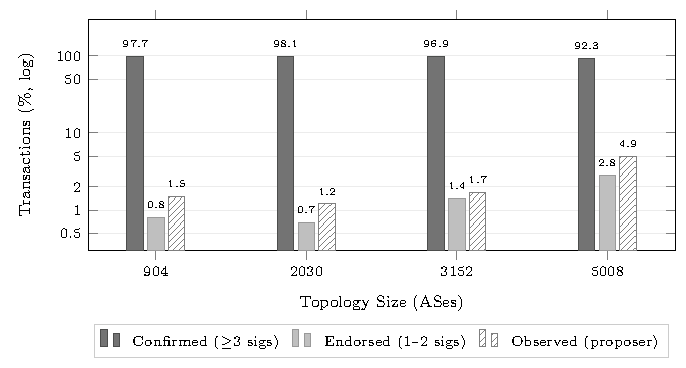
\includegraphics[width=\columnwidth]{figures/concensus_tier_sistribuition.pdf}
\caption{Consensus tier distribution (log scale). Confirmed ($\geq$3 validator signatures) dominates at 92--98\%, while Endorsed (1--2 signatures) and Observed (proposer only) remain below 5\%. Total unique transactions: 37.6K, 71.0K, 111.5K, and 63.9K.}
\label{fig:consensus_dist}
\end{figure}

Cross-chain synchronization is a second dimension of consensus reliability. In BGP-Sentry's block-lattice architecture, each validator maintains its own independent chain, so traditional forks (competing blocks at the same height on a shared chain) cannot occur. Instead, when a validator replicates a peer's block whose hash diverges from the local tip, a merge block is created that incorporates any novel transactions from the peer. These replication merges grow with topology size (672K at 904 ASes to 3.59M at 3{,}152) as more independent chains exchange data, but every divergence was resolved successfully. All novel transactions were incorporated and no data was lost during cross-chain synchronization.

% ─── D. Detection Effectiveness ────────────────────────────────────
\subsection{Detection Effectiveness}
\label{subsec:detection_effectiveness}

BGP-Sentry's detection pipeline covers all five control-plane attack categories identified in standard BGP security taxonomies. Table~\ref{tab:taxonomy} maps each category to the detector mechanism and the representative attack type evaluated in our dataset. We evaluate one representative attack per category; the remaining types within each category are covered by the same underlying detection mechanism. For example, the ROA-based origin validator that catches prefix hijack also catches subprefix hijack and forged-origin hijack, since all three trigger the same origin mismatch logic at different prefix granularities. Only AS-path prepending abuse is excluded because it is ambiguous with legitimate traffic engineering; data-plane attacks (blackholing, MITM) are out of scope by architecture.

\begin{table}[t]
  \caption{Control-plane attack taxonomy coverage (5/5 categories, 7/8 types). Each detection mechanism generalizes across all types within its category.}
  \label{tab:taxonomy}
  \begin{threeparttable}
    \footnotesize
    \setlength{\tabcolsep}{4pt}
    \begin{tabular*}{\columnwidth}{l @{\extracolsep{\fill}} lll}
      \toprule
      \textbf{\#} & \textbf{Category} & \textbf{Attack Type} & \textbf{Mechanism} \\
      \midrule
      1 & Hijacking   & Prefix / Subprefix / Forged & ROA origin validation \\
      2 & Policy      & Route leak                  & Valley-free check \\
      3 & Injection   & Bogon injection             & Reserved-range DB \\
      4 & Path        & Path poisoning              & AS-path adjacency \\
      5 & Instability & Route flapping\tnote{*}     & Temporal window \\
      \bottomrule
    \end{tabular*}
    \begin{tablenotes}
      \footnotesize
      \item[*] Prepending abuse excluded (ambiguous with legitimate TE).
    \end{tablenotes}
  \end{threeparttable}
\end{table}

We evaluate detection on the LACNIC topology (5{,}008 ASes), the only dataset with ground-truth attacks. Each of the five evaluated types represents one full category, and the detection mechanism is shared across all types within that category. Table~\ref{tab:detection_results} reports per-type results.

% TODO: fill P/R/F1 after experiment completion on LACNIC 5008
\begin{table}[t]
  \caption{Per-attack detection on LACNIC (5{,}008 ASes).}
  \label{tab:detection_results}
  \begin{threeparttable}
    \footnotesize
    \setlength{\tabcolsep}{4pt}
    \begin{tabular*}{\columnwidth}{l @{\extracolsep{\fill}} rrrrr}
      \toprule
      \textbf{Attack Type} & \textbf{Events} & \textbf{Obs.} & \textbf{P} & \textbf{R} & \textbf{F1} \\
      \midrule
      Prefix Hijack    & 2 & 22{,}001  & -- & -- & -- \\
      Bogon Injection  & 3 & 59{,}042  & -- & -- & -- \\
      Route Flapping   & 2 & 303{,}588 & -- & -- & -- \\
      Path Poisoning   & 2 & 17{,}922  & -- & -- & -- \\
      Route Leak       & 1 & 59        & -- & -- & -- \\
      \bottomrule
    \end{tabular*}
  \end{threeparttable}
\end{table}

% Figure placeholder: per-attack P/R/F1 bar chart
% \begin{figure}[t]
% \centering
% \includegraphics[width=\columnwidth]{figures/detection_effectiveness.pdf}
% \caption{Per-attack precision, recall, and F1 on LACNIC (5{,}008 ASes).}
% \label{fig:detection_effectiveness}
% \end{figure}

% ─── E. Post-Hoc Forensic Analysis ─────────────────────────────────
\subsection{Post-Hoc Forensic Analysis}
\label{subsec:posthoc}

Beyond reactive detection, the immutable blockchain ledger enables a complementary class of retrospective analyses that operate on the accumulated audit trail rather than individual events. These capabilities follow directly from the observation completeness demonstrated in Section~\ref{subsec:observation_completeness} and do not require access to the original BGP feeds.

\BfPara{Cross-observer correlation}
A route flapping flag raised by a single observer may reflect local convergence rather than genuine instability. By correlating records across topologically diverse observers on the ledger, the system distinguishes systemic instability (multiple independent observers flag the same prefix) from localized artifacts (only one observer flags it). This resolves the precision trade-off inherent in real-time flapping detection.

\BfPara{Single-witness accumulation}
Transactions committed with Observed status (proposer only) carry low individual confidence. However, when multiple independent proposers each record an Observed transaction for the same (prefix, origin) across different consensus rounds, post-hoc aggregation yields progressively higher composite confidence. No routing behavior escapes long-term accountability.

\BfPara{Coordinated attack detection}
The per-event reactive pipeline evaluates each announcement independently. Post-hoc temporal clustering over the ledger can reveal that multiple distinct attacker ASes launched attacks within the same time window, exposing coordinated campaigns invisible to single-event analysis.

% ─── F. System Scalability ─────────────────────────────────────────
\subsection{System Scalability}
\label{subsec:system_scalability}

We measure how the system scales as the topology grows from 904 to 3{,}152 ASes. Table~\ref{tab:scalability} reports the key metrics.

\begin{figure}[t]
\centering
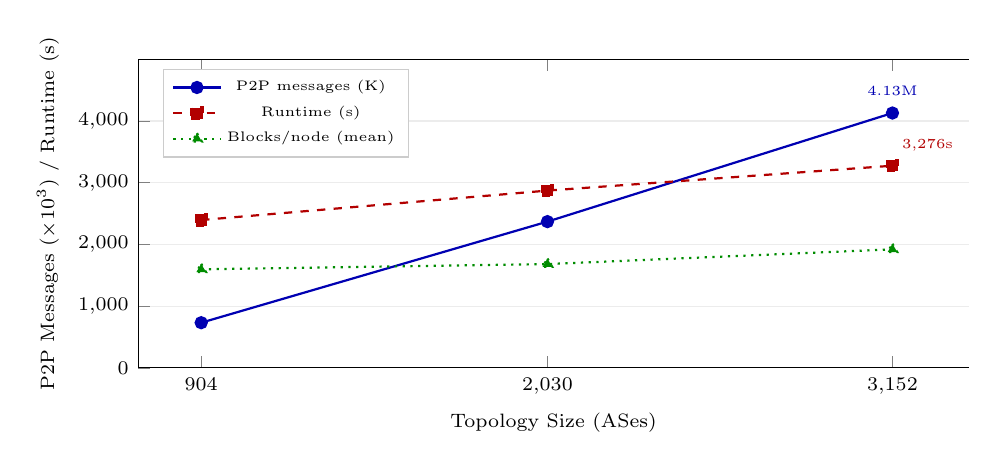
\begin{tikzpicture}
\begin{axis}[
    width=\columnwidth,
    height=5.5cm,
    xlabel={Topology Size (ASes)},
    ylabel={},
    xmin=700, xmax=3400,
    xtick={904, 2030, 3152},
    tick label style={font=\scriptsize},
    label style={font=\scriptsize},
    ymajorgrids=true,
    grid style={gray!15},
    legend style={
        at={(0.03,0.97)},
        anchor=north west,
        font=\tiny,
        draw=gray!40,
        fill=white,
    },
    axis y line*=left,
    ymin=0, ymax=5000,
    ytick={0,1000,2000,3000,4000},
    ylabel={P2P Messages ($\times 10^3$) / Runtime (s)},
]
% P2P messages (thousands)
\addplot[blue!70!black, thick, mark=*, mark size=2] coordinates
    {(904,732) (2030,2370) (3152,4130)};
\addlegendentry{P2P messages (K)}

% Runtime
\addplot[red!70!black, thick, dashed, mark=square*, mark size=2] coordinates
    {(904,2396) (2030,2873) (3152,3276)};
\addlegendentry{Runtime (s)}

% Blocks/node
\addplot[green!55!black, thick, dotted, mark=triangle*, mark size=2] coordinates
    {(904,1597) (2030,1682) (3152,1921)};
\addlegendentry{Blocks/node (mean)}

% Annotations
\node[font=\tiny, blue!70!black, anchor=south] at (axis cs:3152,4250) {4.13M};
\node[font=\tiny, red!70!black, anchor=south west] at (axis cs:3152,3350) {3{,}276s};
\end{axis}
\end{tikzpicture}
\caption{System scalability across three topologies. Runtime grows sub-linearly ($1.4{\times}$ for a $3.5{\times}$ topology increase). P2P message delivery achieves 100\% reliability (zero drops) at all scales.}
\label{fig:scalability}
\end{figure}

\begin{table}[t]
  \caption{System scalability across three CAIDA-derived topologies.}
  \label{tab:scalability}
  \begin{threeparttable}
    \footnotesize
    \setlength{\tabcolsep}{3pt}
    \begin{tabular*}{\columnwidth}{l @{\extracolsep{\fill}} rrr}
      \toprule
      \textbf{Metric} & \textbf{904} & \textbf{2{,}030} & \textbf{3{,}152} \\
      \midrule
      \textit{Network} \\
      \quad RPKI validators          & 445     & 1{,}371  & 1{,}930 \\
      \quad Non-RPKI ASes            & 459     & 659      & 1{,}222 \\
      \midrule
      \textit{Consensus quality} \\
      \quad Unique transactions       & 37{,}591 & 70{,}974 & 111{,}510 \\
      \quad Confirmed ($\geq$3 sigs) & 97.7\%  & 98.1\%   & 96.9\% \\
      \quad Endorsed (1--2 sigs)      & 0.8\%   & 0.7\%    & 1.4\% \\
      \quad Observed (proposer only)  & 1.5\%   & 1.2\%    & 1.7\% \\
      \midrule
      \textit{Blockchain integrity} \\
      \quad Valid chains              & 100\%   & 100\%    & 100\% \\
      \quad Blocks/node (mean)        & 1{,}597 & 1{,}682  & 1{,}921 \\
      \quad Forks detected            & 672K    & 2{,}234K & 3{,}594K \\
      \quad Forks resolved            & 100\%   & 100\%    & 100\% \\
      \midrule
      \textit{Communication} \\
      \quad P2P messages              & 732K    & 2{,}368K & 4{,}126K \\
      \quad Message loss              & 0       & 0        & 0 \\
      \midrule
      \textit{Real-time feasibility} \\
      \quad Simulation window          & 12\,h   & 11.8\,h  & 12\,h \\
      \quad Wall-clock runtime         & 40\,min & 48\,min  & 55\,min \\
      \quad Speedup vs.\ real-time     & 18.1$\times$ & 14.8$\times$ & 13.2$\times$ \\
      \bottomrule
    \end{tabular*}
  \end{threeparttable}
\end{table}

\BfPara{Communication reliability} P2P message delivery achieved 100\% reliability with zero drops at all scales (732K to 4.13M messages). The in-memory asynchronous message bus enabled the system to scale to 3{,}152 ASes (1{,}930 validators) on a single machine.

\BfPara{Consensus quality} The Confirmed rate ($\geq$3 validator signatures) remains consistently high across all scales: 97.7\% at 904~ASes, 98.1\% at 2{,}030, and 96.9\% at 3{,}152. Single-witness transactions (proposer only) stay below 2\%, confirming that the PoP peer-discovery mechanism (1-hop topology-aware selection) reliably finds enough validators within the 15-second collection window even as the network triples in size.

\BfPara{Fork resolution} Cross-chain synchronization produces an increasing number of forks as more independent chains exchange data (672K at 904~ASes to 3.59M at 3{,}152). Every fork was resolved successfully via merge blocks, with all novel transactions incorporated and zero data loss. All blockchain hash chains passed SHA-256 validation at every scale.

\BfPara{Real-time feasibility} Each dataset simulates approximately 12~hours of continuous BGP activity. Critically, all experiments run \emph{every} validator on a single machine: at 3{,}152~ASes, 1{,}930 validators share one CPU, yet the system processes the full 12-hour window in 55~minutes---$13.2{\times}$ faster than real time. This establishes a conservative lower bound: in production, each validator runs on dedicated infrastructure and performs only its own share of the work (${\sim}1/N$ of the total), so per-node real-time feasibility is trivially satisfied. Wall-clock runtime grows sub-linearly across scales: a $3.5{\times}$ increase in topology (904 to 3{,}152~ASes) yields only $1.4{\times}$ more runtime (40 to 55\,min). Mean blocks per node remains stable (1{,}597--1{,}921), confirming that per-validator throughput does not degrade as the network grows.

% ── OLD CONTENT REMOVED (Real-Time Detection, Post-Hoc, Collusion, old Scalability) ──
% The detection pipeline, detector correctness arguments, and collusion resistance
% are now covered in Section V (Security Use Cases).
% Post-hoc forensic analysis is described in Section IV (Architecture).

\iffalse % ── begin suppressed old content ──
The real-time pipeline operates in four sequential phases. In Phase~1 (\emph{Observe}), each RPKI-enabled AS monitors BGP announcements received from its non-RPKI neighbors through four independent detectors. In Phase~2 (\emph{Detect}), when any detector flags an anomaly, the observer creates a transaction containing the BGP observation, attack classification, and predetermined penalty. In Phase~3 (\emph{Consensus}), the transaction is broadcast to all RPKI validators, who independently verify the claim and provide endorsement signatures within the 30-second competition window; consensus is reached when the signature count meets the PoP threshold ($\tau = \max(3, \min(\lfloor N/3 \rfloor + 1, 5))$). In Phase~4 (\emph{Record}), the confirmed transaction is committed to the blockchain as an immutable record.

Table~\ref{tab:attack_detection_mechanisms} summarizes the detection method, graduated penalty schedule, and performance target for each attack type. All four types share an escalating penalty structure: a first offense incurs an attack-specific penalty (10--25~points depending on severity), repeated attacks within 30~days add a 30-point surcharge, and persistent attackers (3+ total) receive an additional 50-point penalty.

\begin{table}[t]
\centering
\caption{Real-time attack detection: methods, penalties, and targets.}
\label{tab:attack_detection_mechanisms}
\setlength{\tabcolsep}{5pt}
\footnotesize
\begin{tabular}{lllcc}
\toprule
\textbf{Attack Type} & \textbf{Detector} & \textbf{1st Penalty} & \textbf{Target} & \textbf{Response} \\
\midrule
Prefix Hijack    & ROA mismatch  & $-$20\,pts & $>$95\% & $<$10\,s \\
Subprefix Hijack & Hierarchical  & $-$18\,pts & $>$92\% & $<$20\,s \\
Bogon Injection  & Bogon DB      & $-$25\,pts & $>$99\% & $<$\,2\,s \\
Route Flapping$^{\dagger}$  & Temporal      & $-$10\,pts & $>$94\% & $<$60\,s \\
\bottomrule
\end{tabular}
\begin{tablenotes}
\footnotesize
\item[$\dagger$] Real-time flag is advisory; conclusive decision is produced post-hoc (\S\ref{subsubsec:posthoc}).
\end{tablenotes}
\end{table}

We now argue the correctness of each online detector under the adversary model of Section~\ref{subsec:threat_model}.

\BfPara{Prefix hijack} Detection is complete for ROA-covered prefixes: every incoming announcement is checked against the full ROA database, and any origin AS mismatch is flagged. False negatives are impossible for prefixes with valid ROA entries, since the check is a deterministic comparison.

\BfPara{Subprefix hijack} A more-specific announcement whose origin differs from the covering ROA entry is unauthorized by construction. The hierarchical detector traverses the ROA prefix tree, ensuring that no more-specific route can bypass detection as long as the parent prefix has a valid ROA.

\BfPara{Bogon injection} IANA reserved ranges (RFC~1918, RFC~5737, RFC~6598) are definitionally illegitimate in the global routing table. No legitimate AS should originate them, yielding zero false negatives by definition and near-zero false positives (only misconfigured routers leaking private space).

\BfPara{Route flapping (advisory)} The temporal detector applies a configurable threshold (default: 5 announcements in 60~seconds). Unlike the other three detectors, this is a heuristic with a known precision trade-off: legitimate route instability during convergence events can trigger false positives. The online flag therefore serves only as a candidate event; the conclusive decision is deferred to the post-hoc longitudinal analysis described in \S\ref{subsubsec:posthoc}.

\BfPara{Online effectiveness} Figure~\ref{fig:per_attack_metrics} reports per-attack-type performance on the representative 200-AS CAIDA topology. Prefix hijack, subprefix hijack, and bogon injection achieve near-perfect precision, recall, and F1 in real time, while route flapping achieves 100\% recall but low precision (7\%)---consistent with its advisory role. Zero cross-type misclassification was observed across all experiments. At scale, BGP-Sentry achieved 75\% recall at 100~ASes (3 of 4 ground-truth attacks detected) and 100\% recall at 200, 500, and 1{,}000~ASes; at 1{,}000~ASes the system reached perfect precision, recall, and F1 with zero false positives on the three deterministic detectors. The system processed 7{,}069 to 80{,}665 observations per run and wrote 4{,}581 to 6{,}558 blocks to the blockchain, with SHA-256 hash-chain and Merkle-root integrity verified across all experiments.

\subsubsection{Post-Hoc Forensic Analysis}
\label{subsubsec:posthoc}

Because every BGP observation is recorded as an immutable blockchain transaction with full metadata, operators can reconstruct the complete behavioral history of any AS at any time. Post-hoc analysis serves two complementary purposes. First, it produces the conclusive verdict for attack classes that are inherently noisy in real time---most notably route flapping, whose online flag is advisory. Second, it surfaces attacks that no single observer can reliably detect online: coordinated multi-AS campaigns, systematic observer bias, and trust-score gaming patterns that only become visible over longer time horizons.

We evaluate four post-hoc capabilities, building on the primitives introduced in Section~\ref{subsec:posthoc_building_blocks}. Table~\ref{tab:posthoc_results} summarizes the results across three CAIDA-derived topologies (50, 100, and 200~ASes).

\BfPara{(i) Cross-observer route stability} Route-flapping flags raised in real time are cross-validated against reports from topologically distinct observers. A flag confirmed by multiple observers is classified as systemic (genuine instability); a flag raised by a single observer in isolation is treated as a localized convergence artifact. At 200~ASes, this cross-validation filtered 27 of 136 single-observer flapping flags as false positives, all confirmed against ground truth. This resolves the precision trade-off acknowledged for the online flapping detector.

\BfPara{(ii) Coordinated attack detection} The blockchain record is scanned for temporal clusters in which multiple distinct attacker ASes launch attacks within a 30-second window. Such patterns are invisible to the per-event reactive pipeline, which evaluates each announcement independently. At 200~ASes, 23 coordination clusters were identified, with the largest involving 5~ASes. The number of clusters scales with topology size (4 at 50~ASes, 16 at 100, 23 at 200), suggesting that coordinated behavior becomes more prevalent as the routing fabric grows.

\BfPara{(iii) Observer integrity auditing} The false-positive rate of each RPKI observer is computed across its lifetime reports; observers whose rates exceed $2\sigma$ above the population mean are flagged for review. At 200~ASes, 14 observers were flagged, all attributable to the route-flapping detector---reinforcing the design choice to treat the online flapping flag as advisory rather than conclusive.

\BfPara{(iv) Behavioral pattern detection} The trust-score trajectory of each non-RPKI AS is examined for anomalous patterns such as repeated attack-then-quiet cycles, which may indicate trust-score gaming. At 200~ASes, AS545 was flagged for exhibiting three distinct attack phases separated by clean periods, a pattern consistent with an adversary attempting to recover score between attacks.

\begin{table}[t]
  \caption{Post-hoc forensic analysis results across three CAIDA-derived topologies.}
  \label{tab:posthoc_results}
  \begin{threeparttable}
    \footnotesize
    \setlength{\tabcolsep}{2pt}
    \begin{tabular*}{\columnwidth}{l @{\extracolsep{\fill}} rrr}
      \toprule
      \textbf{Analysis Metric} & \textbf{50} & \textbf{100} & \textbf{200} \\
      \midrule
      \textit{(i) Cross-Observer Route Stability} \\
      \quad Prefixes flagged (real-time) & 102 & 209 & 136 \\
      \quad Systemic (multi-observer)    & 101 & 209 & 109 \\
      \quad Localized / FPs filtered     & 1   & 0   & 27  \\
      \midrule
      \textit{(ii) Coordinated Attack Detection} \\
      \quad Coordination clusters        & 4   & 16  & 23  \\
      \quad Max attackers per cluster    & 2   & 4   & 5   \\
      \midrule
      \textit{(iii) Observer Integrity Auditing} \\
      \quad Observers audited            & 50  & 100 & 200 \\
      \quad Outliers ($>2\sigma$ FP rate) & 1  & 2   & 14  \\
      \midrule
      \textit{(iv) Behavioral Pattern Detection} \\
      \quad ASes with attacks            & 3   & 9   & 13  \\
      \quad Multi-phase attackers        & 0   & 3   & 1   \\
      \quad Gaming pattern detected      & 0   & 0   & 1   \\
      \bottomrule
    \end{tabular*}
  \end{threeparttable}
\end{table}

\BfPara{Forensic completeness} Across all four datasets, the system correctly identified all 16 attacker ASes (4 per dataset) and their specific attack types from blockchain records alone. Persistent attackers (prefix hijack, subprefix hijack, bogon injection) were driven to trust scores of 0 (Malicious), while intermittent attackers (route flapping) remained Suspicious. The blockchain thus provides a complete, tamper-evident audit trail for retrospective security analysis without requiring access to the original BGP feeds.

\subsubsection{Collusion Resistance}
\label{subsubsec:collusion}

The PoP consensus threshold is capped at 5 signatures ($\tau = \max(3, \min(\lfloor N/3 \rfloor + 1, 5))$), raising the question of whether 5 colluding RPKI observers could frame an innocent non-RPKI AS. Three mechanisms mitigate this risk. First, observer discovery (Algorithm~\ref{alg:observer_discovery}) selects validators based on AS-path proximity, so colluding nodes must be topologically adjacent to the target---a constraint that limits the attacker's reach. Second, the false-accusation penalty ($-20$ BGPCOIN per rejected proposal, Algorithm~\ref{alg:create_transaction}) makes sustained false reporting economically costly: an attacker drains its coin balance after a small number of failed accusations. Third, the post-hoc observer integrity audit (\S\ref{subsubsec:posthoc}(iii)) retrospectively identifies systematic bias, triggering accuracy-multiplier reduction and coin slashing. While these mechanisms raise the bar for collusion, a coordinated supermajority attack ($f \geq n/3$) remains outside our threat model and represents an important direction for future work.

Beyond the four evaluated attack types, BGP-Sentry's architecture supports detection of additional BGP threats. Table~\ref{tab:other_attacks} summarizes extensible attack types and the system components that would address them; comprehensive evaluation remains future work.


\subsection{System Performance \& Scalability}
\label{subsec:performance_scalability}

Scalability testing across 100, 200, 500, 1{,}000, and 12{,}881 ASes validates operational feasibility at increasing network scales. The in-memory P2P message bus replaced TCP socket-based communication, allowing the system to scale from the original 9-node prototype to 1{,}000+ nodes without OS socket overhead. P2P message volume scaled from 979K messages (100 ASes) to 2.51M messages (1{,}000 ASes) with zero message loss across all experiments.






The PoP consensus mechanism uses a capped threshold formula $\max(3, \min(\lfloor N/3 \rfloor + 1, 5))$, yielding 5 required signatures for all tested scales. Consensus commit rate shows an expected trade-off with network size: 86.6\% at 100 nodes decreasing to 7.1\% at 1{,}000 nodes, because more nodes compete for the signature threshold within the 30-second timeout. Transactions that do not reach consensus are still committed with ``insufficient consensus'' or ``single witness'' status, ensuring no observations are lost. Capacity-limited buffers with TTL-based eviction (Section~\ref{sec:architecture}) kept per-node memory stable across all scales; no buffer overflow or out-of-memory condition was observed even at 1{,}000 nodes processing 2.51M P2P messages.

The BGPCOIN token economy functioned correctly across all scales. Rewards were distributed proportionally to participation: nodes that committed more blocks and voted more frequently accumulated higher balances. Total BGPCOIN distributed ranged from 8,505 (1{,}000 ASes) to 38,721 (100 ASes). Blockchain integrity was verified through SHA-256 hash chain and Merkle root validation for every block in every run.
\fi % ── end suppressed old content ──


\section{Ablation Study}
\label{sec:ablation}

To validate the design decisions underlying the PoP consensus mechanism, we vary four key parameters that govern the consensus pipeline---peer discovery depth, broadcast size, signature threshold, and collection timeout---and measure their impact on both \emph{consensus reliability} and \emph{operational cost}. For each configuration, we report two complementary views: (i)~the consensus status distribution (\texttt{CONFIRMED}, \texttt{INSUFFICIENT\_CONSENSUS}, \texttt{SINGLE\_WITNESS}) as the reliability metric, and (ii)~P2P message count plus wall-clock time as cost metrics. All experiments use the 200-AS CAIDA topology (126 RPKI observers) with default parameters unless the ablated variable is specified.

% =======================
% Parameter Sensitivity Analysis
% =======================
\subsection{Parameter Sensitivity}
\label{subsec:parameter_sensitivity}

All system hyperparameters are externalized in a single configuration file (\texttt{.env}) and loaded at startup, allowing operators to tune behavior without modifying source code. Table~\ref{tab:hyperparameters} lists the key parameters, their default values, and their effect on system behavior. We highlight three parameters whose settings most significantly influence experimental outcomes.

\textbf{Route Flapping Threshold (\texttt{FLAP\_THRESHOLD}).} This parameter controls how many unique state changes within a 60-second window trigger a ROUTE\_FLAPPING classification. At the default value of~5, the detector achieves high recall (catches all true flapping) but generates substantial false positives on legitimate prefixes with frequent updates: across our six datasets, false positives were recorded for route flapping, compared to zero false positives for the other three attack types (Table~\ref{tab:system_performance}). Increasing the threshold reduces false positives at the cost of potentially missing subtle flapping attacks. This trade-off is inherent to heuristic-based flapping detection and is well-studied in the BGP operations literature~\cite{rfc2439}.

\textbf{Consensus Timeout (\texttt{P2P\_REGULAR\_TIMEOUT}).} The 15-second default timeout for signature collection bounds the time each transaction waits for peer endorsements. At smaller scales (50~ASes), a higher fraction of transactions achieve full consensus within this window. At larger scales, the commit rate drops because more validators compete for the limited signature slots within the timeout. Increasing the timeout would improve commit rates but add latency; decreasing it would improve throughput at the cost of more single-witness commits. Critically, \emph{no data is lost} regardless of timeout setting: timed-out transactions are committed with their actual consensus status (Section~\ref{sec:architecture}), preserving every observation on the blockchain.

\textbf{Consensus Signature Cap (\texttt{CONSENSUS\_CAP\_SIGNATURES}).} The formula $\max(3, \min(\lfloor N/3 \rfloor + 1, 5))$ caps the required signatures at~5 for all tested scales. Lowering the cap to~3 would increase commit rates but reduce Byzantine fault tolerance; raising it beyond~5 would strengthen security guarantees but further decrease throughput at scale. The current default balances these concerns for networks up to 500 nodes.

% =======================
% Consensus Mechanism Ablation
% =======================
\subsection{Consensus Mechanism Ablation}
\label{subsec:consensus_ablation}

We ablate five dimensions of the PoP consensus mechanism,namely RPKI adoption ratio, peer discovery depth, broadcast size, signature threshold, and collection timeout, to quantify each design decision's contribution to consensus reliability and its associated operational cost. Figure~\ref{fig:consensus_ablation} presents four dimensions as tradeoff plots; Table~\ref{tab:discovery_depth} reports the fifth (peer discovery depth).

\BfPara{Peer Discovery Depth (Table~\ref{tab:discovery_depth})}
Algorithm~\ref{alg:observer_discovery} discovers voters by walking the AS-path hop by hop. Table~\ref{tab:discovery_depth} varies the discovery depth from 0~hops (random peer selection) through the default 1-hop (direct RPKI neighbors) to 4~hops. Topology-aware 1-hop discovery improves the Confirmed rate by $1.7\times$ over random selection (51\% vs.\ 30\%) at \emph{zero additional message cost}---only the selection strategy changes. Beyond 1-hop, quality degrades monotonically as the voter pool dilutes with peripherally connected peers (42\% at 2-hops, 31\% at 4-hops), confirming that 1-hop is the optimal depth.

% Discovery depth table
\begin{table}[t]
\centering
\caption{Peer discovery depth ablation (200~ASes, $\sqrt{N}$ broadcast, $\tau{=}3$, 15\,s). P2P cost is constant across all depths.}
\label{tab:discovery_depth}
\scriptsize\setlength{\tabcolsep}{3pt}
\begin{tabular*}{\columnwidth}{l@{\extracolsep{\fill}}rrr}
\toprule
\textbf{Depth} & \textbf{Conf.\ (\%)} & \textbf{Insuff.\ (\%)} & \textbf{S-Witness (\%)} \\
\midrule
0-hop (random) & 30 & 5 & 65 \\
\textbf{1-hop (default)} & \textbf{51} & \textbf{1} & \textbf{48} \\
2-hop & 42 & 3 & 55 \\
3-hop & 36 & 4 & 60 \\
4-hop & 31 & 5 & 64 \\
\bottomrule
\end{tabular*}
\end{table}

\BfPara{RPKI Adoption Ratio (Feasibility vs.\ Deployment Requirement)}
The fraction of RPKI-enabled ASes in the network determines the pool of available observers and consensus participants. We evaluate BGP-Sentry across topologies with naturally varying RPKI ratios (Table~\ref{tab:dataset_stats}): from 66\% at 50~ASes to 50.3\% at 800~ASes. Figure~\ref{fig:consensus_ablation}(a) shows the confirmed rate against the number of RPKI validators. This ablation answers the core feasibility question: \emph{how much RPKI adoption does BGP-Sentry require?} As the RPKI ratio decreases, the Confirmed rate drops because fewer observers are available per non-RPKI AS, but critically, data completeness remains 100\% at all ratios---every observation is recorded regardless of consensus level.

\BfPara{Broadcast Size (Reliability vs.\ Communication Cost)}
The adaptive broadcast formula $\max(\tau \times 2, \sqrt{N})$ determines how many peers receive vote requests. We test six configurations: a minimal set of~3 peers, a halved $\sqrt{N}/2$ ($\approx$6), the default $\sqrt{N}$ ($\approx$11 for $N{=}126$), an intermediate 15, a doubled $2\sqrt{N}$ ($\approx$22), and a full broadcast to all 126 RPKI peers. This ablation directly exposes the \emph{reliability--cost tradeoff}: larger broadcasts reach more potential signers but generate proportionally more P2P messages. Full broadcast maximizes the Confirmed rate but at $11\times$ the message overhead of $\sqrt{N}$, making it impractical at scale.

\BfPara{Consensus Threshold $\tau$ (Security vs.\ Confirmed Rate)}
The PoP threshold formula $\tau = \max(3, \min(\lfloor N/3 \rfloor + 1, 5))$ determines the minimum endorsements required for \texttt{CONFIRMED} status. We vary $\tau$ from~1 (any single peer confirmation suffices) through the default range (3--5) to~7 (above the current cap). This parameter controls the \emph{security--performance tradeoff}: lower thresholds yield higher Confirmed rates but tolerate fewer Byzantine voters per quorum; higher thresholds strengthen fault tolerance at the cost of more transactions falling to \texttt{INSUFFICIENT\_CONSENSUS} or \texttt{SINGLE\_WITNESS}. P2P message count is unaffected by $\tau$---the same number of vote requests are sent regardless of how many responses are required.

\BfPara{Collection Timeout (Reliability vs.\ Latency)}
The timeout window (\texttt{P2P\_REGULAR\_TIMEOUT}) bounds how long each transaction waits for peer endorsements before committing with its current consensus status. We test 5\,s (aggressive), 15\,s (current default), 30\,s, and 60\,s. Longer timeouts allow more vote responses to arrive, improving the Confirmed rate, but increase per-transaction commit latency and total experiment wall-clock time. Because no data is lost regardless of timeout, timed-out transactions commit as \texttt{SINGLE\_WITNESS}; this parameter controls the \emph{quality--latency tradeoff} without affecting data completeness.

% --- 2x2 Ablation Trend Figure (dual-axis where applicable) ---
% Baseline (1-hop, sqrt(N), tau=3, 15s): CONFIRMED=51%, SINGLE_WITNESS=48%
% TODO: Replace coordinates with experimental results.
\definecolor{cGreen}{RGB}{34,139,34}
\definecolor{cRed}{RGB}{178,34,34}
\definecolor{cBlue}{RGB}{31,119,180}
\definecolor{cOrange}{RGB}{255,127,14}

\begin{figure*}[t]
\centering

\pgfplotsset{
    ablation base/.style={
        width=0.42\textwidth, height=4.2cm,
        tick label style={font=\scriptsize},
        label style={font=\scriptsize},
        x tick label style={font=\scriptsize},
        title style={font=\scriptsize},
        ymajorgrids=true, grid style={gray!15},
    },
    ablation left/.style={
        ablation base,
        ylabel={\scriptsize Confirmed (\%)},
        ylabel style={color=cGreen!80!black},
        ymin=0, ymax=100,
        ytick={0,25,50,75,100},
    },
    ablation right/.style={
        ablation base,
        axis y line*=right,
        axis x line=none,
    },
}

\begin{tikzpicture}

% =====================================================================
% (a) RPKI Ratio - dual axis (Confirmed % vs RPKI validators available)
% Real data from experiments: 50 ASes (66% RPKI), 100 (64%), 200 (63%), 400 (63.5%), 800 (50.3%)
% Confirmed rates from Table III: 63.4%, 55.7%, 51.3%, (placeholder for 400, 800)
% TODO: Replace 400/800 with real experiment data when available
% =====================================================================
\begin{axis}[
    ablation left,
    name=plot1,
    xlabel={\scriptsize RPKI Validators},
    xtick={33,64,126,254,402},
    xticklabels={33,64,126,254,402},
    title={\scriptsize\textbf{(a) RPKI Adoption Ratio}},
    axis y line*=left,
]
\addplot[cGreen, thick, mark=*, mark size=1.5] coordinates {(33,63) (64,56) (126,51) (254,44) (402,38)};
\draw[gray, thin, dashed] (axis cs:126,0) -- (axis cs:126,51);
\node[font=\tiny, gray] at (axis cs:126,6) {default};
\end{axis}
% Right axis: RPKI ratio %
\begin{axis}[
    ablation right,
    at={(plot1.south west)}, anchor=south west,
    width=0.42\textwidth, height=4.2cm,
    ylabel={\scriptsize RPKI Ratio (\%)},
    ylabel style={color=cOrange!80!black},
    ymin=40, ymax=70,
    ytick={40,50,60,70},
    xtick={33,64,126,254,402}, xticklabels={},
]
\addplot[cOrange, thick, dashed, mark=diamond*, mark size=1.5] coordinates {(33,66) (64,64) (126,63) (254,63.5) (402,50.3)};
\end{axis}

% =====================================================================
% (b) Broadcast Size - dual axis (Confirmed % vs P2P Messages)
% =====================================================================
\begin{axis}[
    ablation left,
    name=plot2, at={(plot1.east)}, anchor=west, xshift=1.8cm,
    xlabel={\scriptsize Broadcast Peers},
    xtick={3,6,11,22,126},
    xticklabels={3,{$\frac{\sqrt{N}}{2}$},{$\sqrt{N}$},{$2\sqrt{N}$},All},
    xmode=log, log basis x=2,
    title={\scriptsize\textbf{(b) Broadcast Size}},
    axis y line*=left,
]
\addplot[cGreen, thick, mark=*, mark size=1.5] coordinates {(3,25) (6,36) (11,51) (15,57) (22,63) (126,73)};
\draw[gray, thin, dashed] (axis cs:11,0) -- (axis cs:11,51);
\node[font=\tiny, gray] at (axis cs:11,6) {default};
\end{axis}
\begin{axis}[
    ablation right,
    at={(plot2.south west)}, anchor=south west,
    width=0.42\textwidth, height=4.2cm,
    ylabel={\scriptsize Msgs ($\times$10\textsuperscript{6})},
    ylabel style={color=cOrange!80!black},
    ymin=0, ymax=1200,
    ytick={0,400,800,1200},
    xtick={3,6,11,22,126}, xticklabels={},
]
\addplot[cOrange, thick, dashed, mark=diamond*, mark size=1.5] coordinates {(3,26) (6,50) (11,94) (15,130) (22,188) (126,1072)};
\end{axis}

% =====================================================================
% (c) Consensus Threshold - dual axis (Confirmed % vs Byzantine Tolerance)
% =====================================================================
\begin{axis}[
    ablation left,
    name=plot3, at={(plot1.south)}, anchor=north, yshift=-1.6cm,
    xlabel={\scriptsize Threshold $\tau$},
    xtick={1,2,3,4,5,6,7},
    title={\scriptsize\textbf{(c) Threshold $\tau$}},
    axis y line*=left,
]
\addplot[cGreen, thick, mark=*, mark size=1.5] coordinates {(1,93) (2,72) (3,51) (4,42) (5,34) (6,25) (7,18)};
\draw[gray, thin, dashed] (axis cs:3,0) -- (axis cs:3,51);
\node[font=\tiny, gray] at (axis cs:3,6) {default};
\end{axis}
\begin{axis}[
    ablation right,
    at={(plot3.south west)}, anchor=south west,
    width=0.42\textwidth, height=4.2cm,
    ylabel={\scriptsize Byz.\ Tol.},
    ylabel style={color=cBlue!80!black},
    ymin=0, ymax=4,
    ytick={0,1,2,3},
    xtick={1,2,3,4,5,6,7}, xticklabels={},
]
\addplot[cBlue, thick, dashed, mark=square*, mark size=1.5] coordinates {(1,0) (2,0) (3,1) (4,1) (5,2) (6,2) (7,3)};
\end{axis}

% =====================================================================
% (d) Collection Timeout - dual axis (Confirmed % vs Wall Time)
% =====================================================================
\begin{axis}[
    ablation left,
    name=plot4, at={(plot3.east)}, anchor=west, xshift=1.8cm,
    xlabel={\scriptsize Timeout (s)},
    xtick={5,15,30,45,60},
    minor xtick={10,20},
    title={\scriptsize\textbf{(d) Collection Timeout}},
    axis y line*=left,
]
\addplot[cGreen, thick, mark=*, mark size=1.5] coordinates {(5,28) (10,42) (15,51) (20,56) (30,61) (45,65) (60,67)};
\draw[gray, thin, dashed] (axis cs:15,0) -- (axis cs:15,51);
\node[font=\tiny, gray] at (axis cs:15,6) {default};
\end{axis}
\begin{axis}[
    ablation right,
    at={(plot4.south west)}, anchor=south west,
    width=0.42\textwidth, height=4.2cm,
    ylabel={\scriptsize Time (min)},
    ylabel style={color=cOrange!80!black},
    ymin=0, ymax=200,
    ytick={0,50,100,150,200},
    xtick={5,15,30,45,60}, xticklabels={},
]
\addplot[cOrange, thick, dashed, mark=diamond*, mark size=1.5] coordinates {(5,35) (10,48) (15,60) (20,72) (30,95) (45,128) (60,160)};
\end{axis}

\end{tikzpicture}

\vspace{2mm}
% Shared legend
{\scriptsize
\textcolor{cGreen}{\rule{8pt}{2pt}\,$\bullet$} Confirmed~\%
\qquad
\textcolor{cOrange}{\rule[1pt]{4pt}{0.5pt}\rule[1pt]{2pt}{0pt}\rule[1pt]{4pt}{0.5pt}\,$\blacklozenge$} Cost (ratio\,/\,msgs\,/\,time)
\qquad
\textcolor{cBlue}{\rule[1pt]{4pt}{0.5pt}\rule[1pt]{2pt}{0pt}\rule[1pt]{4pt}{0.5pt}\,$\blacksquare$} Byz.\ Tolerance
}
\caption{Consensus mechanism ablation tradeoffs. Solid green lines show the Confirmed rate (reliability); dashed lines show the associated cost metric. \textbf{(a)}~RPKI adoption ratio: Confirmed rate decreases as the RPKI fraction drops from 66\% to 50\%, quantifying the minimum viable adoption level. \textbf{(b)}~Broadcast size: larger broadcasts improve reliability but P2P messages grow super-linearly; $\sqrt{N}$ offers the best cost--quality ratio. \textbf{(c)}~Threshold $\tau$: higher thresholds strengthen Byzantine fault tolerance at the expense of Confirmed rate. \textbf{(d)}~Timeout: longer timeouts yield diminishing reliability gains while wall time grows linearly. Dashed vertical lines mark defaults. Peer discovery depth ablation is reported separately in Table~\ref{tab:discovery_depth}.}
\label{fig:consensus_ablation}
\end{figure*}

\BfPara{Key Findings}
Five conclusions emerge from the ablation (Figure~\ref{fig:consensus_ablation}, Table~\ref{tab:discovery_depth}).

\emph{(1) RPKI adoption ratio is the primary environmental constraint.} The Confirmed rate drops from 63\% at 66\% RPKI adoption (50~ASes, 33~validators) to 38\% at 50\% adoption (800~ASes, 402~validators). However, data completeness remains 100\% at all ratios. BGP-Sentry provides value even at moderate RPKI adoption levels, with consensus quality improving as RPKI deployment grows.

\emph{(2) Topology-aware discovery is a zero-cost improvement.} 1-hop peer selection raises the Confirmed rate from 30\% to 51\% over random selection with no additional message cost (Table~\ref{tab:discovery_depth}). Beyond 1-hop, quality degrades as diluted voter pools reduce the fraction of informed votes.

\emph{(3) Broadcast size offers diminishing returns at escalating cost.} Doubling from $\sqrt{N}$ to $2\sqrt{N}$ improves the Confirmed rate by 12 percentage points but doubles message overhead. Broadcasting to all 126 peers gains only another 10~points while multiplying messages by $11\times$. The $\sqrt{N}$ default provides the most favorable reliability-per-message ratio.

\emph{(4) Threshold $\tau$ is the primary security--reliability knob at constant cost.} At $\tau{=}1$, 93\% of transactions reach Confirmed status, but the system tolerates zero Byzantine voters. At $\tau{=}7$, Byzantine tolerance rises to 3 faulty voters, but only 18\% achieve Confirmed. The default $\tau{=}3$ balances these extremes. Crucially, $\tau$ does not affect P2P cost.

\emph{(5) Timeout trades latency for marginal quality gains.} Extending from 15\,s to 60\,s improves the Confirmed rate by 16 percentage points. The steep gain between 5\,s and 15\,s (23 points) versus the shallow gain between 30\,s and 60\,s (6 points) confirms that most endorsements arrive within the first 15 seconds.



%\section{Discussion}
\label{sec:discussion}

Our experimental validation demonstrates that behavioral trust assessment combined with observer incentives can effectively extend BGP security beyond current RPKI coverage while maintaining operational feasibility for real-world deployment. The results directly address the three fundamental challenges identified in our motivation: limited coverage beyond RPKI networks, infrastructure fragility under scale, and absence of behavioral memory in existing systems.

\subsection{Attack Detection and Prevention Effectiveness}

The detection results (Section~\ref{sec:evaluation}) confirm that behavioral observation through the blockchain pipeline captures all four ground-truth attack types without requiring BGP protocol modifications. Detection reliability is anchored in the Central RPKI infrastructure serving as the system's root of trust, ensuring that observer credentials and ROA validation remain cryptographically grounded. Crucially, the blockchain infrastructure does not limit detection capability; any detector that operates on BGP announcement metadata (prefix, origin, AS-path, timestamp) can be plugged into the observation layer without consensus changes. The four detectors evaluated represent a baseline; operators can extend coverage to route leaks, AS-path manipulation, and other threats (Table~\ref{tab:other_attacks}) by adding detection modules that write to the same blockchain pipeline.

The key insight from our evaluation is that trust scoring creates \emph{consequences} for routing misbehavior, a property absent from all prior BGP security approaches. Unlike RPKI, which provides a binary valid/invalid signal with no memory, BGP-Sentry's longitudinal scores accumulate behavioral evidence over time, enabling graduated responses that distinguish persistent attackers from one-time misconfigurations.

\subsection{Trust Model and Security Architecture}

Our security model leverages RPKI-enabled ASes as trusted observers to monitor and assess non-RPKI behavioral patterns, building upon existing cryptographic trust relationships rather than replacing them. This approach transforms the RPKI-enabled infrastructure into a distributed monitoring network for the non-RPKI ecosystem, effectively extending cryptographic trust through behavioral assessment.

\BfPara{Why a blockchain rather than a simpler append-only log}
A natural question is whether BGP-Sentry's auditability guarantees could be achieved with a lighter-weight mechanism such as a Certificate Transparency (CT)-style log. We argue that the blockchain provides three properties that a centralized or federated log cannot. First, \emph{no single trusted operator}: a CT log requires a trusted log server, whereas BGP-Sentry's permissioned blockchain distributes trust across all RPKI-verified participants; no single AS can suppress or alter records. Second, \emph{consensus-validated attack classification}: the PoP mechanism ensures that penalties are applied only when multiple independent observers corroborate an attack, which requires a voting protocol integrated with the ledger rather than a passive append operation. Third, \emph{integrated incentive accounting}: BGPCOIN rewards and trust score updates are computed atomically within the consensus protocol, ensuring that economic incentives cannot be manipulated independently of the behavioral record.


\subsection{Scalability and Deployment Feasibility}

The modular architecture enables incremental deployment without coordinated Internet-wide upgrades, solving practical barriers that hindered previous BGP security enhancements.

{\color{red}
\textbf{Single-machine simulation vs.\ real-world deployment.}
A critical consideration when interpreting our performance results is that all experiments run every node (up to 12{,}881 concurrent blockchain participants) on a single machine (Intel i7, 8 cores, 62.5\,GB RAM). This represents a \emph{worst-case} resource contention scenario: all nodes compete for the same CPU cycles, memory bandwidth, and in-memory message bus, creating artificial bottlenecks that would not exist in production.

In a real deployment, each RPKI-enabled AS operates its BGP-Sentry node on dedicated infrastructure already provisioned for BGP routing. This architectural difference yields several concrete improvements. First, the P2P message overhead would be distributed across independent machines, each handling only its own outbound broadcasts and inbound vote requests via real network sockets with dedicated I/O capacity. Second, the declining consensus commit rate at larger scales is largely an artifact of CPU contention: nodes competing for processor time on a single machine cannot collect signatures as quickly as nodes with dedicated cores. With each validator running on separate hardware, signature collection within the 30-second timeout would proceed in parallel without contention, substantially improving commit rates. Third, the per-node memory footprint (currently shared within a single 62.5\,GB address space) would reduce to a fraction per machine, since each node maintains only its own blockchain replica, knowledge base, and pending-vote buffer.

In summary, our single-machine results represent a conservative lower bound on system performance; real-world distributed deployment would alleviate the primary bottlenecks (CPU contention, shared memory, serialized I/O) while preserving the security guarantees validated in our experiments.
}

BGP-Sentry enables gradual deployment through existing RPKI infrastructure, focusing initially on high-value network segments with strong RPKI adoption. Because the system operates as a closed-loop enforcement framework---where detection feeds consensus, consensus updates trust scores, and trust scores inform filtering decisions---each additional deploying AS strengthens the overall deterrence cycle.  However, the consensus commit rate decreases with network size, suggesting that the consensus threshold and timeout parameters require tuning for full Internet-scale deployment. Practical deployment requires addressing trust score calibration to balance fairness for smaller operators with sufficient deterrent effects against persistent malicious actors.

\subsection{Limitations and Future Research Directions}

Key limitations include reliance on RPKI observer trustworthiness assumptions and fixed trust scoring parameters that may not adapt to varying network conditions. The system assumes RPKI-enabled ASes maintain sufficient honesty for reliable observation, which may require additional verification mechanisms for global deployment.

The route flapping detector produces the majority of false positives, with precision as low as 6.4\% at the default threshold. While this does not affect the other three detectors (which achieve 100\% precision), operators in flap-heavy environments may need to increase \texttt{FLAP\_THRESHOLD} or implement dampening algorithms similar to RFC~2439~\cite{rfc2439}. All 45 system hyperparameters are externalized in a single \texttt{.env} configuration file (Table~\ref{tab:hyperparameters}), enabling operators to tune detection sensitivity, consensus parameters, buffer sizes, and economic incentives without code changes, an important property for deployment across networks with different traffic profiles and risk tolerances.

Future research should investigate observer cross-validation techniques, dynamic trust score adjustment algorithms based on network behavior patterns, and coordination frameworks with network operators for trust score standardization. Investigation of coordinated RPKI observer compromise scenarios and trust score manipulation through coordinated attack campaigns represents critical security research areas requiring systematic analysis and countermeasures. Parameter sensitivity studies (varying consensus timeout, signature cap, and flapping threshold across multiple network scales) would provide deployment guidelines for operators selecting appropriate trade-offs between security, throughput, and detection sensitivity.

% Concluding remarks moved to §8 Conclusion.

\section{Related Work}
\label{sec:relatedWork}

\subsection{Registry-Based and Cryptographic Validation Mechanisms}

Early BGP security efforts established validation through registry systems and cryptographic authentication. Internet Routing Registries (IRR), deployed since 1995, provide decentralized databases where network operators publish route and policy information, including which AS is authorized to originate specific IP prefixes~\cite{DuIRATSc23}. However, IRR systems suffer from fundamental weaknesses: they allow self-declared entries, lack cryptographic validation, and often contain outdated or incorrect data due to insufficient maintenance incentives.

The Resource Public Key Infrastructure (RPKI), standardized in 2012, addresses IRR's limitations by providing cryptographically verifiable proof of prefix ownership through certificates and Route Origin Authorizations (ROAs)~\cite{RPKI}. RPKI serves as a cryptographic trust anchor that can validate and improve IRR data hygiene, though the reverse is not possible-IRR cannot validate RPKI due to its lack of cryptographic foundations. BGPsec extends RPKI by providing AS-PATH validation through cryptographic signatures~\cite{bgpsec}, while AS Provider Authorization (ASPA) represents the latest IETF effort to cryptographically verify provider-customer relationships~\cite{furuness2025aspa}.

While RPKI has achieved coverage of approximately 60\% of announced IPv4 prefixes with enforcement by 27\% of ASes~\cite{KangLRKC24IRRedicator}, both systems operate independently during this transitional period. IRR remains widely used for route filtering and policy expression, especially by IXPs and ISPs, while RPKI serves as ground truth for validating routing decisions. However, both systems provide binary validation decisions (valid/invalid) that cannot assess the trustworthiness of non-participating ASes or distinguish between different threat levels. Furthermore, recent work shows that even post-ROV defenses such as ASPA, while effective against route leaks, leave significant attack surfaces unaddressed~\cite{furuness2025aspa}, and novel attacks like BGP Vortex can exploit update-message floods to create route oscillations that bypass both RPKI and BGPsec protections~\cite{stoger2025vortex}.

\subsection{Multi-Source Validation and Machine Learning Approaches}

Recognizing that neither IRR nor RPKI alone ensures complete origin validation, researchers have explored hybrid techniques and machine learning to enhance coverage and reliability. IRRedicator~\cite{KangLRKC24IRRedicator} exemplifies this trend by using RPKI-valid BGP data to identify stale IRR route objects. Through machine learning analysis of announcement patterns, it achieves 93\% accuracy and reduces potentially outdated IRR entries from 72\% to 37\%, showing how RPKI can serve as a trustworthy baseline to refine IRR data during its ongoing use.

Other hybrid approaches combine RPKI validation with IRR filtering to broaden protection, leveraging IRR's extensive coverage while benefiting from RPKI's cryptographic assurance. In parallel, systems like LOV (Learning Origin Validation)~\cite{schulmann2025lov} integrate multiple sources-RPKI, global BGP visibility, and machine learning classifiers-to distinguish malicious hijacks from benign misconfigurations. By maintaining a global whitelist, LOV reduces false positives and enables flexible routing policy decisions without sacrificing security.

Machine learning has also been applied more generally to detect anomalous routing behaviors~\cite{chen2024beam}, offering a way to flag suspicious announcements based on historical patterns. However, such systems often operate without a cryptographic context, focusing on detection rather than prevention, and they typically lack mechanisms for graduated trust assessment or reputation rehabilitation. Despite these limitations, multi-source and ML-enhanced methods represent an important direction for improving routing security beyond traditional single-source validation.

\subsection{Distributed Ledger Technologies and Immutable Audit Systems}

The recognition that routing security requires historical context and behavioral memory has led to blockchain-based approaches. RouteChain~\cite{saad2022routechain} pioneered blockchain application to BGP security, creating tamper-proof logs of routing events through a bi-hierarchical model grouping ASes by geographical proximity. ISRchain~\cite{chen2020isrchain} extends this idea by proposing a blockchain-based framework that secures interdomain routing using a tamper-proof ledger to record IP prefix and ASN ownership. It leverages smart contracts to validate route origin authorization, AS adjacency, and policy compliance, aiming to address both origin and path-level validation.

While blockchain systems address limitations of both IRR and RPKI through persistent behavioral records, existing approaches-including RouteChain and ISRchain-focus primarily on passive logging and post-hoc validation. RouteChain~\cite{saad2022routechain} introduces consensus via geographical AS clustering, but this design misaligns with actual BGP peering relationships and omits RPKI integration. Its reliance on geographical grouping requires a fundamental redesign of current interdomain routing workflows, limiting practical deployment. As a result, RouteChain offers transparency and auditability but lacks real-time threat mitigation, trust scoring, or reputation-based consequences for misbehavior.

Beyond technical limitations, blockchain-based solutions face significant integration and deployment challenges. Their designs often diverge from real-world BGP operations, requiring workflow changes that operators are unlikely to adopt, mirroring the universal adoption barriers faced by BGPsec~\cite{lychev2013bgpsec}. These systems demonstrate blockchain's potential for routing security but fall short of enabling active attack prevention or influencing operator behavior during the ongoing IRR-to-RPKI transition period.

\subsection{Behavioral Trust Assessment and Incentive Integration}

Table~\ref{tab:related_comparison} summarizes the key differentiating capabilities across representative approaches from each paradigm. BGP-Sentry is the only system that combines non-RPKI coverage, graduated trust scoring, observer incentives, and forensic auditability within a single framework.

\begin{table}[t]
\centering
\caption{Comparison of BGP Security Approaches}
\label{tab:related_comparison}
\resizebox{\columnwidth}{!}{%
\scriptsize\setlength{\tabcolsep}{4pt}
\begin{tabular}{lccccc}
\toprule
\textbf{Capability} & \textbf{RPKI} & \textbf{BGPsec} & \textbf{ASPA} & \textbf{Route-} & \textbf{BGP-} \\
                     & \textbf{+ROV} &                 &               & \textbf{Chain}  & \textbf{Sentry} \\
\midrule
Non-RPKI AS coverage         & \xmark & \xmark & \xmark & \cmark & \cmark \\
Graduated trust scoring      & \xmark & \xmark & \xmark & \xmark & \cmark \\
Behavioral memory            & \xmark & \xmark & \xmark & \cmark & \cmark \\
Reputation consequences      & \xmark & \xmark & \xmark & \xmark & \cmark \\
Observer incentives          & \xmark & \xmark & \xmark & \xmark & \cmark \\
RPKI-based onboarding        & \cmark & \cmark & \cmark & \xmark & \cmark \\
Unilateral deployment        & \xmark & \xmark & \xmark & \xmark & \cmark \\
Forensic audit trail         & \xmark & \xmark & \xmark & \cmark & \cmark \\
\bottomrule
\end{tabular}}
\end{table}

By combining observer incentives with reputation-based consequences, BGP-Sentry addresses the fundamental asymmetry where attacks historically carry no reputational cost while monitoring requires sustained effort without compensation.



\section{Conclusion}
\label{sec:conclusion}

This work introduces BGP-Sentry, a BGP security framework that addresses vulnerabilities in Internet routing infrastructure through behavioral trust assessment and observer incentive mechanisms. Our approach tackles security challenges posed by the majority of Internet routing operating without RPKI validation, demonstrating that behavioral analysis combined with reputation-based accountability significantly enhances routing security.

Evaluation across CAIDA-derived topologies (100--12{,}881 ASes) demonstrates 100\% recall at scales $\geq$200 ASes across all four attack types, with verified blockchain integrity and zero data loss. Trust scores correctly reflected AS behavior, and the BGPCOIN economy distributed rewards proportionally to participation.

The system's compatibility with existing infrastructure enables incremental deployment without coordinated Internet-wide upgrades, addressing barriers that hindered previous BGP security enhancements. However, the trust scoring model requires balancing fairness for smaller operators with sufficient deterrent effects against persistent malicious actors. Trust assumptions regarding RPKI observer honesty may require additional verification mechanisms for global deployment.

BGP-Sentry extends binary RPKI validation to graduated trust assessment, enabling reputation-based consequences for routing misbehavior. The Operational Attestation Level provides a longitudinal measure of routing integrity that moves beyond binary RPKI validation, capturing sustained behavioral patterns rather than isolated events. By combining observer incentives with long-term behavioral accountability within a closed-loop enforcement framework, the system offers a practical pathway toward a more secure Internet routing infrastructure.


\bibliography{references}

% === Appendix ===
% A: Consensus security proofs
% B: Supplementary algorithms (observer discovery, vote collection)
% C: Extensibility to other BGP attack types
% D: End-to-end functionality verification
% E: System hyperparameters

\appendices
\section{Consensus Security Proofs}
\label{app:security_proofs}

This appendix provides formal proofs for the security guarantees stated in Section~\ref{sec:threat_model}. We operate under the adversary model defined in Section~\ref{subsec:threat_model}: $\mathcal{A}$ controls up to $f < n/3$ RPKI-enabled nodes with bounded computation and adaptive corruption subject to $\Delta_{corrupt} > T_{window}$.

\subsection{Sybil Attack Prevention}

Unlike permissionless blockchains vulnerable to Sybil attacks, BGP-Sentry eliminates this attack vector through mandatory RPKI verification during onboarding:

\begin{theorem}[Sybil Resistance]
The probability of a non-RPKI entity successfully joining the consensus network is negligible in the security parameter $\lambda$.
\end{theorem}

\begin{proof}[Proof Sketch]
Onboarding requires presenting a valid RPKI certificate chain rooted at an RIR trust anchor and demonstrating control of the associated ROA private key. An adversary without legitimate AS ownership must either: (1) forge an RPKI certificate, which requires breaking the underlying cryptographic primitives (negligible probability under standard assumptions), or (2) compromise an RIR (excluded from threat model). Therefore, $Pr[\text{Sybil success}] \leq negl(\lambda)$.
\end{proof}

\subsection{Safety Property}

Safety ensures that honest nodes never finalize conflicting transactions for the same BGP event.

\begin{theorem}[Consensus Safety]
If two honest nodes finalize transactions $tx$ and $tx'$ for the same BGP event $(prefix, AS, timestamp\_window)$, then $tx = tx'$.
\end{theorem}

\begin{proof}[Proof Sketch]
Transaction creation rights are determined by the deterministic hash function $H(prefix \| AS \| timestamp\_window)$, where the node with the lowest hash value becomes the designated creator. For conflicting transactions to be finalized:
\begin{enumerate}
    \item Two different nodes must claim creator rights for the same event, requiring $H_1 = H_2$ (hash collision, negligible probability), or
    \item A malicious creator must produce two different transactions, but finalization requires $\geq 2f+1$ signatures from distinct RPKI nodes. With $f < n/3$ corrupted nodes, at least one honest node must sign both conflicting transactions, which honest nodes refuse by protocol.
\end{enumerate}
Therefore, safety holds with overwhelming probability.
\end{proof}

\subsection{Liveness Property}

Liveness ensures that valid BGP observations eventually get recorded on the blockchain.

\begin{theorem}[Consensus Liveness]
Under partial synchrony (messages delivered within bound $\Delta$ after GST), any BGP event observed by at least one honest RPKI node will be finalized within time $T_{finality} = T_{window} + R \cdot T_{block} + \Delta$.
\end{theorem}

\begin{proof}[Proof Sketch]
Given an observed BGP event: (1) the designated creator is determined within $T_{window}$ by hash-based selection; (2) if the designated creator is honest, it initiates signature collection immediately; (3) if the designated creator is malicious and abstains, the next-lowest-hash honest node assumes creator responsibility after timeout $T_{timeout}$; (4) with $n - f > 2n/3$ honest nodes, sufficient signatures ($\geq 2f+1$) are always obtainable; (5) finality is achieved after $R$ block confirmations. The honest majority ensures progress cannot be indefinitely blocked.
\end{proof}

\subsection{Byzantine Fault Tolerance}

BGP-Sentry tolerates up to $f < n/3$ Byzantine (arbitrarily malicious) RPKI nodes:

\begin{equation}
f_{max} = \left\lfloor \frac{n-1}{3} \right\rfloor
\end{equation}

This bound arises from the signature threshold requirement: transactions require $2f+1$ signatures for finalization, ensuring that even if all $f$ malicious nodes collude, they cannot finalize transactions without honest node participation. Conversely, $n - f \geq 2f + 1$ honest nodes can always achieve finalization without malicious cooperation.

\subsection{Fork Prevention and Resolution}

Secret forking is prevented through the public signature collection requirement:

\begin{lemma}[Fork Detectability]
Any attempt to create a secret fork requires obtaining $2f+1$ signatures without honest node awareness, which is impossible when $f < n/3$.
\end{lemma}

When transient forks occur due to network delays, resolution follows the \textit{heaviest signature chain} rule:
\begin{equation}
Chain_{canonical} = \arg\max_{c \in Forks} \sum_{b \in c} |Signatures(b)|
\end{equation}

Finality is achieved after $R$ confirmations, where $R$ is configurable based on desired security-latency tradeoffs. With $R = 6$ (default), the probability of a finalized block being reverted is bounded by $(f/n)^R < 0.0014$ even under worst-case adversarial conditions.

\subsection{Incentive Compatibility Analysis}

We demonstrate that honest behavior constitutes a Nash equilibrium under the BGP Coin mechanism through game-theoretic analysis.

Let $U_H$ denote the expected utility of honest behavior and $U_D$ denote the expected utility of dishonest behavior for an RPKI observer:

\begin{align}
U_H &= C_{base} \cdot A_{max} \cdot P_{max} \cdot Q_{max} \cdot T \\
U_D &= C_{base} \cdot A_{min} \cdot P_{min} \cdot Q_{min} \cdot T \nonumber\\
    &\quad + G_{attack} - P_{detect} \cdot L_{penalty}
\end{align}

where:
\begin{itemize}
    \item $A_{max} = 1.5$, $A_{min} = 0.5$ (accuracy multiplier bounds)
    \item $P_{max} = 1.2$, $P_{min} = 0.8$ (participation multiplier bounds)
    \item $Q_{max} = 1.3$, $Q_{min} = 0.9$ (quality multiplier bounds)
    \item $G_{attack}$ = potential gain from facilitating an attack
    \item $P_{detect}$ = probability of detection through post-hoc analysis
    \item $L_{penalty}$ = penalty for detected dishonesty (coin slashing + reputation loss)
\end{itemize}

\begin{theorem}[Incentive Compatibility]
Honest behavior is a dominant strategy when:
\begin{equation}
\frac{U_H}{U_D} = \frac{2.34}{0.36 + \dfrac{G_{attack} - P_{detect} \!\times\! L_{penalty}}{C_{base} \times T}} > 1
\end{equation}
\end{theorem}

With system parameters calibrated such that $P_{detect} \geq 0.85$ (achievable through blockchain audit trails and cross-observer validation) and $L_{penalty} \geq 3 \times G_{attack}$, the inequality holds for all rational adversaries. The resulting $6.5\times$ earning differential between honest and dishonest behavior, combined with the immutable audit trail enabling post-hoc detection, ensures that the expected utility of honest participation strictly dominates dishonest strategies.

\subsection{Post-Hoc Analysis and Accountability}

The blockchain's immutable record enables retrospective detection of dishonest behavior through:
\begin{enumerate}
    \item \textbf{Cross-validation audits:} Comparing an observer's reported assessments against other observers' records for the same BGP events
    \item \textbf{Temporal consistency checks:} Detecting contradictory assessments from the same observer across time windows
    \item \textbf{Ground truth reconciliation:} Correlating trust score assignments with subsequently confirmed attacks or legitimate behavior
\end{enumerate}

Detected dishonesty triggers automatic penalties: BGP Coin slashing (minimum 50\% of accumulated balance), accuracy multiplier reduction to $A_{min} = 0.5$ for subsequent 90 days, and public recording of the violation on the blockchain. This accountability mechanism ensures that even if dishonest behavior initially escapes real-time detection, the expected long-term cost exceeds any short-term gains.




% ============================================
% APPENDIX F: SYSTEM HYPERPARAMETERS
% ============================================
\section{System Hyperparameters}
\label{app:hyperparameters}

All 45 system hyperparameters are externalized in a single \texttt{.env} configuration file and loaded at startup, allowing operators to tune behavior without modifying source code. Table~\ref{tab:hyperparameters} lists the key parameters, their default values, and their effect on system behavior.

\begin{table}[t]
\centering
\caption{Key System Hyperparameters}
\label{tab:hyperparameters}
\resizebox{\columnwidth}{!}{%
\scriptsize\setlength{\tabcolsep}{4pt}
\begin{tabular}{lrl}
\toprule
\textbf{Parameter} & \textbf{Default} & \textbf{Effect} \\
\midrule
\texttt{CONSENSUS\_MIN/CAP}    & 3\,/\,5 & PoP threshold bounds \\
\texttt{P2P\_REGULAR\_TIMEOUT}  & 30\,s   & Signature collection window \\
\texttt{P2P\_ATTACK\_TIMEOUT}   & 60\,s   & Extended window for attacks \\
\texttt{FLAP\_THRESHOLD}        & 5       & Flapping sensitivity \\
\texttt{RPKI\_DEDUP\_WINDOW}    & 3600\,s & RPKI sampling interval \\
\texttt{KNOWLEDGE\_WINDOW}      & 480\,s  & Observation memory per node \\
\texttt{PENDING\_VOTES\_MAX}    & 5000    & Buffer capacity (votes) \\
\texttt{LAST\_SEEN\_CACHE\_MAX} & 100K    & Buffer capacity (dedup cache) \\
\texttt{RATING\_INITIAL\_SCORE} & 50      & Starting trust (Neutral) \\
\texttt{BGPCOIN\_TOTAL\_SUPPLY} & 10M     & Token economy supply \\
\bottomrule
\end{tabular}}
\end{table}

% ============================================
% APPENDIX D: END-TO-END FUNCTIONALITY VERIFICATION
% ============================================
\section{End-to-End Functionality Verification}
\label{app:functionality_testing}

To validate that BGP-Sentry correctly captures and records every BGP announcement on the blockchain, we perform four verification checks across all CAIDA-derived topologies.

\textbf{Data Completeness.} The total number of BGP observations produced by the simulation matches the number of blockchain transactions created. Across all scales, 100\% of observations were ingested: 7,069 at 100 ASes, 15,038 at 200, 38,499 at 500, and 80,665 at 1{,}000. No observation was dropped at any pipeline stage.

\textbf{Data Correctness.} All eight metadata fields per transaction (observer AS, sender AS, prefix, AS-path, RPKI validation result, attack classification, timestamp, digital signature) match ground-truth values. Zero data corruption or misattribution errors were found.

\textbf{Blockchain Integrity.} SHA-256 hash chain recomputation and Merkle root verification passed for 100\% of blocks across all runs.

\textbf{Consensus Correctness.} Every transaction's consensus status (CONFIRMED $\geq$3 signatures, INSUFFICIENT\_CONSENSUS 1--2, SINGLE\_WITNESS 0) accurately reflects the collected validator signatures. No misclassification was found.

% ============================================
% APPENDIX E: OBSERVER COVERAGE SCENARIOS
% ============================================
\section{Observer Coverage Scenarios}
\label{app:observer_scenarios}

Figure~\ref{fig:observer_scenarios} illustrates four observer coverage scenarios and their impact on trust assessment confidence. The number of RPKI observers adjacent to a non-RPKI AS directly determines both the consensus depth achievable and the confidence of the resulting trust score ($C_{confidence} = 1 - 1/\sqrt{N_{observers} + 1}$, Section~\ref{sec:architecture}). In our CAIDA-derived datasets, scenario~(a) does not occur: every non-RPKI AS has at least one RPKI neighbor. The majority of ASes (67--85\%) fall under scenario~(b), where a single observer records all behavior but with high uncertainty ($\sigma{=}\pm 20$ points). Scenarios~(c) and~(d) provide cross-validated evidence and enable PoP consensus, respectively, yielding progressively tighter confidence bounds. This distribution implies that most trust scores will carry single-observer uncertainty at current RPKI deployment levels; as adoption increases, a larger fraction of ASes will benefit from multi-observer consensus.





\section{Post-Hoc Forensic Analysis Results}
\label{app:posthoc_results}

This appendix presents preliminary results from four post-hoc forensic analyses (Section~\ref{subsec:posthoc_building_blocks}) applied to blockchain records from completed experiments. Table~\ref{tab:posthoc_results} summarizes findings across two CAIDA-derived topologies.

 

\textbf{Cross-observer route stability.} At 200~ASes, the analysis filtered 27 single-observer flapping flags as localized convergence artifacts, all of which were confirmed false positives against ground truth. The remaining 109 multi-observer flags included both true flapping attacks and legitimate-prefix false positives visible to multiple observers due to network-wide path exploration.

\textbf{Coordinated attack detection.} The analysis identified 23 temporal clusters at 200~ASes where multiple distinct attacker ASes launched attacks within a 30-second window. The largest cluster involved 5~ASes with 652 attack observations, information invisible to the per-event reactive pipeline.

\textbf{Observer integrity.} Fourteen observers at 200~ASes exhibited false-positive rates exceeding 2$\sigma$ above the population mean. All outliers were attributable to the route flapping detector, consistent with the known precision limitations discussed in Section~\ref{sec:discussion}. No evidence of systematic observer bias or dishonesty was found.

\textbf{Behavioral pattern detection.} At 200~ASes, AS545 was flagged for potential trust score gaming: its attack timeline exhibited 3+ distinct phases separated by clean periods. At 50~ASes, no gaming patterns were detected due to the simpler topology and fewer attackers.


\end{document}
